% ******************************* PhD Thesis Template **************************
% Please have a look at the README.md file for info on how to use the template

\documentclass[letterpaper,12pt,times,oneside,numbered,print,index,custommargin,PageStyleI]{Classes/PhDThesisPSnPDF}

% ******************************************************************************
% ******************************* Class Options ********************************
% *********************** See README for more details **************************
% ******************************************************************************

% `a4paper'(The University of Cambridge PhD thesis guidelines recommends a page
% size a4 - default option) or `a5paper': A5 Paper size is also allowed as per
% the Cambridge University Engineering Deparment guidelines for PhD thesis
%
% `11pt' or `12pt'(default): Font Size 10pt is NOT recommended by the University
% guidelines
%
% `oneside' or `twoside'(default): Printing double side (twoside) or single
% side.
%
% `print': Use `print' for print version with appropriate margins and page
% layout. Leaving the options field blank will activate Online version.
%
% `index': For index at the end of the thesis
%
% `draftclassic': For draft mode without loading any images (same as draft in book)
%
% `draft': Special draft mode with line numbers, images, and water mark with
% timestamp and custom text. Position of the text can also be modified.
%
% `abstract': To generate only the title page and abstract page with
% dissertation title and name, to submit to the Student Registry
%
% `chapter`: This option enables only the specified chapter and it's references
%  Useful for review and corrections.
%
% ************************* Custom Page Margins ********************************
%
% `custommargin`: Use `custommargin' in options to activate custom page margins,
% which can be defined in the preamble.tex. Custom margin will override
% print/online margin setup.
%
% *********************** Choosing the Fonts in Class Options ******************
%
% `times' : Times font with math support. (The Cambridge University guidelines
% recommend using times)
%
% `fourier': Utopia Font with Fourier Math font (Font has to be installed)
%            It's a free font.
%
% `customfont': Use `customfont' option in the document class and load the
% package in the preamble.tex
%
% default or leave empty: `Latin Modern' font will be loaded.
%
% ********************** Choosing the Bibliography style ***********************
%
% `authoryear': For author-year citation eg., Krishna (2013)
%
% `numbered': (Default Option) For numbered and sorted citation e.g., [1,5,2]
%
% `custombib': Define your own bibliography style in the `preamble.tex' file.
%              `\RequirePackage[square, sort, numbers, authoryear]{natbib}'.
%              This can be also used to load biblatex instead of natbib
%              (See Preamble)
%
% **************************** Choosing the Page Style *************************
%
% `default (leave empty)': For Page Numbers in Header (Left Even, Right Odd) and
% Chapter Name in Header (Right Even) and Section Name (Left Odd). Blank Footer.
%
% `PageStyleI': Chapter Name next & Page Number on Even Side (Left Even).
% Section Name & Page Number in Header on Odd Side (Right Odd). Footer is empty.
%
% `PageStyleII': Chapter Name on Even Side (Left Even) in Header. Section Number
% and Section Name in Header on Odd Side (Right Odd). Page numbering in footer

% Uncomment to change page style
%\pagestyle{PageStyleII}

\usepackage[spanish,english]{babel}
% ********************************** Preamble **********************************
% Preamble: Contains packages and user-defined commands and settings
% ******************************************************************************
% ****************************** Custom Margin *********************************

% Add `custommargin' in the document class options to use this section
% Set {innerside margin / outerside margin / topmargin / bottom margin}  and
% other page dimensions
\ifsetCustomMargin
  \RequirePackage[left=30mm,right=20mm,top=20mm,bottom=20mm]{geometry}
  \setFancyHdr % To apply fancy header after geometry package is loaded
\fi

% Add spaces between paragraphs
%\setlength{\parskip}{0.5em}
% Ragged bottom avoids extra whitespaces between paragraphs
\raggedbottom
% To remove the excess top spacing for enumeration, list and description
%\usepackage{enumitem}
%\setlist[enumerate,itemize,description]{topsep=0em}

% *****************************************************************************
% ******************* Fonts (like different typewriter fonts etc.)*************

% Add `customfont' in the document class option to use this section

\ifsetCustomFont
  % Set your custom font here and use `customfont' in options. Leave empty to
  % load computer modern font (default LaTeX font).
  %\RequirePackage{helvet}

  % For use with XeLaTeX
  %  \setmainfont[
  %    Path              = ./libertine/opentype/,
  %    Extension         = .otf,
  %    UprightFont = LinLibertine_R,
  %    BoldFont = LinLibertine_RZ, % Linux Libertine O Regular Semibold
  %    ItalicFont = LinLibertine_RI,
  %    BoldItalicFont = LinLibertine_RZI, % Linux Libertine O Regular Semibold Italic
  %  ]
  %  {libertine}
  %  % load font from system font
  %  \newfontfamily\libertinesystemfont{Linux Libertine O}
\fi

% *****************************************************************************
% **************************** Custom Packages ********************************
\usepackage{bm}
\usepackage{bbm}
\usepackage{amsfonts}
\usepackage{amsmath}
\usepackage{amssymb}
\usepackage{float}
\usepackage{siunitx} % use this package module for SI units
%\RequirePackage{amstext}
%\RequirePackage{amsbsy}
%\RequirePackage{amsopn}
%\RequirePackage{gensymb}
%\RequirePackage[cmex10]{amsmath}
\RequirePackage[sumlimits,cmex10]{mathtools}
%\usepackage[sumlimits]{mathtools}
\usepackage{cancel}
%\renewcommand\CancelColor{\color{darkblue}}
%\renewcommand\CancelColor{\color{lightred}}
\usepackage{minted}

\newcommand{\op}{\wedge}

\newcommand{\field}[1]{\mathbb{#1}} % requires amsfonts
\newcommand{\pd}[2]{\frac{\partial#1}{\partial#2}}

\newcommand{\vecbi}[1]{\boldsymbol{#1}}
\renewcommand{\vec}[1]{\bm{#1}}
\newcommand{\pp}{\mathbbm{P}}
\newcommand{\rr}{\mathbbm{R}}
\newcommand{\sss}{\mathbbm{S}}
\newcommand{\Aa}{\mathbb{a}}
\newcommand{\bb}{\mathbb{b}}
\newcommand{\cc}{\mathbb{c}}
\newcommand{\dd}{\mathbb{d}}
\newcommand{\xx}{\mathbbm{x}}
\newcommand{\sv}{\mathbbm{s}}
\newcommand{\av}{\mathbbm{a}}
\newcommand{\bv}{\mathbbm{b}}
\newcommand{\cv}{\mathbbm{c}}
\newcommand{\dv}{\mathbbm{d}}
\newcommand{\uv}{\mathbbm{u}}
\newcommand{\yy}{\mathbb{y}}
\newcommand{\vv}{\mathbb{v}}
\newcommand{\pl}{\mathbb{p}}
\newcommand{\nn}{\mathbb{n}}
\newcommand{\pipi}{\mathbbm{\Pi}}
\newcommand{\ts}{\mathbbm{T}}
%\DeclareMathSizes{10}{10}{7}{5}
%\DeclareMathSizes{11}{11}{7.7}{5.5}
%\DeclareMathSizes{12}{12}{8.4}{6}
%\DeclareMathSizes{13}{13}{9.1}{6.5}
%\DeclareMathSizes{14}{14}{9.8}{7}

% ************************* Algorithms and Pseudocode **************************

%\usepackage{algpseudocode}


% ********************Captions and Hyperreferencing / URL **********************

% Captions: This makes captions of figures use a boldfaced small font.
%\RequirePackage[small,bf]{caption}

\RequirePackage[labelsep=space,tableposition=top]{caption}
\renewcommand{\figurename}{Fig.} %to support older versions of captions.sty


% *************************** Graphics and figures *****************************

%\usepackage{rotating}
%\usepackage{wrapfig}

% Uncomment the following two lines to force Latex to place the figure.
% Use [H] when including graphics. Note 'H' instead of 'h'
%\usepackage{float}
%\restylefloat{figure}

% Subcaption package is also available in the sty folder you can use that by
% uncommenting the following line
% This is for people stuck with older versions of texlive
%\usepackage{sty/caption/subcaption}
\usepackage{subcaption}

% ********************************** Tables ************************************
\usepackage{booktabs} % For professional looking tables
\usepackage{multirow}

%\usepackage{multicol}
%\usepackage{longtable}
%\usepackage{tabularx}


% *********************************** SI Units *********************************
\usepackage{siunitx} % use this package module for SI units


% ******************************* Line Spacing *********************************

% Choose linespacing as appropriate. Default is one-half line spacing as per the
% University guidelines

% \doublespacing
% \onehalfspacing
% \singlespacing


% ************************ Formatting / Footnote *******************************

% Don't break enumeration (etc.) across pages in an ugly manner (default 10000)
%\clubpenalty=500
%\widowpenalty=500

%\usepackage[perpage]{footmisc} %Range of footnote options


% *****************************************************************************
% *************************** Bibliography  and References ********************

%\usepackage{cleveref} %Referencing without need to explicitly state fig /table

% Add `custombib' in the document class option to use this section
\ifuseCustomBib
   \RequirePackage[square, sort, numbers, authoryear]{natbib} % CustomBib

% If you would like to use biblatex for your reference management, as opposed to the default `natbibpackage` pass the option `custombib` in the document class. Comment out the previous line to make sure you don't load the natbib package. Uncomment the following lines and specify the location of references.bib file

%\RequirePackage[backend=biber, style=numeric-comp, citestyle=numeric, sorting=nty, natbib=true]{biblatex}
%\bibliography{References/references} %Location of references.bib only for biblatex

\fi

% changes the default name `Bibliography` -> `References'
%\renewcommand{\bibname}{References}


% ******************************************************************************
% ************************* User Defined Commands ******************************
% ******************************************************************************

%% *********** To change the name of Table of Contents / LOF and LOT ************
%
%\renewcommand{\chaptername}{Capítulo}
%\renewcommand{\contentsname}{Table de Contenidos}
%\renewcommand{\listfigurename}{Lista de Figuras}
%\renewcommand{\listtablename}{Lista de Tablas}
%% changes the default name `Bibliography` -> `References'
%\renewcommand{\bibname}{Bibliografía}

% ********************** TOC depth and numbering depth *************************

\setcounter{secnumdepth}{3}
\setcounter{tocdepth}{3}


% ******************************* Nomenclature *********************************

% To change the name of the Nomenclature section, uncomment the following line

%\renewcommand{\nomname}{Symbols}


% ********************************* Appendix ***********************************

% The default value of both \appendixtocname and \appendixpagename is `Appendices'. These names can all be changed via:

%\renewcommand{\appendixtocname}{List of appendices}
%\renewcommand{\appendixname}{Appndx}

% *********************** Configure Draft Mode **********************************

% Uncomment to disable figures in `draft'
%\setkeys{Gin}{draft=true}  % set draft to false to enable figures in `draft'

% These options are active only during the draft mode
% Default text is "Draft"
%\SetDraftText{DRAFT}

% Default Watermark location is top. Location (top/bottom)
%\SetDraftWMPosition{bottom}

% Draft Version - default is v1.0
%\SetDraftVersion{v1.1}

% Draft Text grayscale value (should be between 0-black and 1-white)
% Default value is 0.75
%\SetDraftGrayScale{0.8}


% ******************************** Todo Notes **********************************
%% Uncomment the following lines to have todonotes.

%\ifsetDraft
%	\usepackage[colorinlistoftodos]{todonotes}
%	\newcommand{\mynote}[1]{\todo[author=kks32,size=\small,inline,color=green!40]{#1}}
%\else
%	\newcommand{\mynote}[1]{}
%	\newcommand{\listoftodos}{}
%\fi

% Example todo: \mynote{Hey! I have a note}

\usepackage{nomencl}
\makenomenclature


% ************************ Thesis Information & Meta-data **********************
% Thesis title and author information, refernce file for biblatex
\crest{
\includegraphics[width=0.2\textwidth]{University_Crest}}
\university{UNIVERSIDAD SIMÓN BOLÍVAR}
\dept{DECANATO DE ESTUDIOS PROFESIONALES\\COORDINACIÓN DE INGENIERÍA DE LA COMPUTACIÓN}

% ************************ Thesis Information & Meta-data **********************
%% The title of the thesis
\title{Implementación de un motor de juego en lenguajes puramente funcionales}
%\texorpdfstring is used for PDF metadata. Usage:
%\texorpdfstring{LaTeX_Version}{PDF Version (non-latex)} eg.,
%\texorpdfstring{$sigma$}{sigma}

%% Subtitle (Optional)
%\subtitle{Using the CUED template}

%% The full name of the author
\author{José Daniel Duran Toro}



%% You can redefine the submission text:
% Default as per the University guidelines:
% ``This dissertation is submitted for the degree of''
\renewcommand{\submissiontext}{Trabajo Especial de Grado \\
para obtener el título de \\
~~ \\%
 }

%% Full title of the Degree
\degreetitle{Ingeniero de la Computación}

%% College affiliation (optional)
%\college{King's College}

%% Submission date
% Default is set as {\monthname[\the\month]\space\the\year}
\degreedate{Sartenejas, Enero 2018}

%% Meta information
\subject{GameEngine} \keywords{{Game Engine} {Haskell} {Functional Programming} {Universidad Simón Bolívar}}


% ***************************** Abstract Separate ******************************
% To printout only the titlepage and the abstract with the PhD title and the
% author name for submission to the Student Registry, use the `abstract' option in
% the document class.

\ifdefineAbstract
 \pagestyle{empty}
 \includeonly{Declaration/declaration, Abstract/abstract}
\fi

% ***************************** Chapter Mode ***********************************
% The chapter mode allows user to only print particular chapters with references
% Title, Contents, Frontmatter are disabled by default
% Useful option to review a particular chapter or to send it to supervisior.
% To use choose `chapter' option in the document class



% ******************************** Front Matter ********************************

\begin{document}
\selectlanguage{spanish}
\lstset{
basicstyle =\scriptsize,          % print whole listing small
keywordstyle =\color{black}\bfseries, % underlined bold black keywords  basicstyle=\ttfamily,
  columns=fullflexible,
  frame=single,
  breaklines=true,
  postbreak=\mbox{\textcolor{red}{$\hookrightarrow$}\space},
}

\frontmatter

\graphicspath{{Figs/}}
\begin{titlepage}

\begin{figure}[!htbp!]
\centering

\includegraphics[width=0.2\textwidth]{University_Crest}
\end{figure}

\begin{center}

\Large UNIVERSIDAD SIMÓN BOLÍVAR\\
\large \textbf {DECANATO DE ESTUDIOS PROFESIONALES}\\
\large \textbf {COORDINACIÓN DE INGENIERÍA DE LA COMPUTACIÓN}\\

\vfill
\large \textbf {BLOCKCHAIN: TECNOLOGÍA DE LIBROS CONTABLES DIGITALES}

\vfill
Por:\\
Alfredo A. Delgado L.

\vfill
Realizado con la asesoría de:\\
Victor Theoktisto y Yudith Cardinale

\vfill
\large PROYECTO DE GRADO\\
Presentado ante la Ilustre Universidad Simón Bolívar\\
como requisito parcial para optar al título de\\
Ingeniero de la Computación

\vfill
\textbf {Sartenejas, Mayo 2018}

\end{center}

\end{titlepage}

% *********** To change the name of Table of Contents / LOF and LOT ************

%\renewcommand{\chaptername}{Capítulo}
%\renewcommand{\contentsname}{Índice de Contenidos}
%\renewcommand{\listfigurename}{Lista de Figuras}
%\renewcommand{\listtablename}{Lista de Tablas}
%% changes the default name `Bibliography` -> `References'
%\renewcommand{\bibname}{Bibliografía}
%\renewcommand{\abstractname}{Resumen}
%\renewcommand{\abstractname}{Resumen}
%\include{Dedication/dedication}
%\include{Declaration/declaration}
%\include{Acknowledgement/acknowledgementa}
% ************************** Thesis Abstract *****************************
% Use `abstract' as an option in the document class to print only the titlepage and the abstract
\begin{abstract}

La tecnología de libros contables distribuidos mejor conocida como \textit{blockchain}, tiene como objetivo, permitir el  registro distribuido e inmutable de transacciones entre entidades. Esta tecnología disruptiva ha empezado a tomar auge en los últimos años, más aún, en sectores o rubros que se distancian mucho de su uso o necesidad inicial (las criptomonedas). El campo educativo no es la excepción; no es difícil proyectar la cantidad de posibilidades que puede ofrecer una tecnología que garantice  inmutabilidad, verificación de identidades y auditoría en tiempo real de cualquier tipo de operación. Sus casos de uso se extienden desde cadena de suministros,  gestión estatal, sistema de votaciones y hasta el rastreo de encomiendas, solo por nombrar algunos de ellos.

%\textcolor{blue}{CORRECCIÓN SUGUERIDA: Afinación final del resumen. Hablar de sigpae}

Entendiendo el gran valor  que esta tecnología puede proveer, es menester de la academia aborse a su estudio e investigación. El presente proyecto, aunado a la creación del Grupo de Investigación Blockchain de la Universidad Simón Bolívar, tiene como finalidad dar inicio a la exploración e investigación de las distintas plataformas \textit{blockchain} existentes, populares y estables; evaluar casos de uso que sean de interés para la Universidad y, por consiguiente, para el grupo de investigación y posteriormente realizar un prototipo  funcional  que simula un proceso de transcripción de programas de estudio y cuyo objetivo es explorar características del \textit{blockchain} beneficiosas y pertinentes a incluir en el Sistema de Gestión de Programas  Analíticos de Estudios (SIGPAE) de la Universidad Simón Bolívar, que se encuentra actualmente en desarrollo  y sera responsable de la ejecución de todos los procesos necesarios para lograr la transcripción efectiva del contenido programático de una materia o curso y posteriormente lograr su inclusión dentro de los programas avalados. Finalmente en este contexto, en este documento se presenta la evaluación de 2 tecnologías \textit{blockchain} (\textit{Ethereum Platform} e \textit{IBM Hyperledger}),su comparación y  justificación  de selección  de \textit{IBM Hyperledger Fabric} para su uso en el desarrollo del prototipo funcional mencionado. Los procesos expuestos dan el punto de partida e inspiración para la demostración propuesta en este trabajo.

%\textcolor{red}{Escribir blockchain en todo el documento como \textit{blockchain}}

%\textcolor{red}{El resumen la vamos a revisar al final. Hay que mencionar el caso de uso que se modela}

\textbf{Palabras clave:} Cadenas de bloque, Contratos inteligentes, Criptografía, Libros Distribuidos, Descentralización.

\end{abstract}

\chapter{Agradecimientos}


Este proyecto de grado en la Universidad Simón Bolívar es un esfuerzo en el cual directa o indirectamente participaron distintas personas ,opinando, corrigiendo, dando animo, o acompañándome en los momentos de crisis y felicidad.
Este trabajo me ha permitido aprovechar la  competencia y la experiencia de muchas personas que deseo agradecer en este apartado.

En primer lugar, a mis tutores Prof. Yudith Cardinale y Prof. Victor Theoktisto, mi mas amplio agradecimiento por toda la paciencia, atención y guía durante todo el desarrollo de este proyecto haciendo posible llegar a la completitud y conclusiones del mismo.

A mis padres Derly y Oswaldo mi eterno agradecimiento por el amor, apoyo, educación, valores y apoyo incondicional recibido durante toda mi vida, lo cual fue pieza clave para terminar esta difícil pero excitante carrera.

Un especial agradecimiento a mi amor y compañera Giuli, quien motivo directamente la realización de este proyecto de grado y aparte de realizar variadas revisiones y correcciones, brindo su apoyo incondicional, moral y emocional en los momentos mas difíciles y complejos de este trabajo. 

A mis amigos de carrera Oriana, Hector, Michelle, Daniel, Andres y Dayana  que directa o indirectamente llegaron a completar mi perfil profesional gracias a sus consejos, aprendizajes y enseñanzas a lo largo de esta carrera sirviendo de  motivación para realizar este proyecto de grado.

A mi amigo de infancia, licenciado Carlos, gracias especiales por su tiempo en la corrección y validación de este proyecto de grado.

Finalmente a mis amigos fraternales de La Cuspide, Luis, Gabriel, Alejandro,Carlitos y Manuel, gracias por todo su apoyo y acompañamiento en esta largo pero gratificante trayecto.

A todos ustedes mi mayor reconocimiento y gratitud.



% *********************** Adding TOC and List of Figures ***********************


\tableofcontents
\listoffigures

\listoftables


% \printnomenclature[space] space can be set as 2em between symbol and description
%\printnomenclature[3em]


% ******************************** Main Matter *********************************
\mainmatter

\chapter{Introducción}
\label{capitulo1}

La tecnología \texti{blockchain} está mayormente asociada al sector financiero y ha saltado a la palestra gracias a la aparición de las criptomonedas. Sin embargo,  empieza a despertar el interés de otros sectores, los cuales buscan aprovechar los beneficios que un registro distribuido e inmutable puede proveerles. Integridad, transparencia y confiabilidad son algunas de las características principales que hacen que las organizaciones, empresas y academias volteen su mirada hacia ella.

El presente trabajo busca exponer las características de la tecnología  \texti{blockchain} y cómo estas pueden ser utilizadas en beneficio de organizaciones que no necesariamente deben relacionarse al sector financiero. Para lograr un mayor entendimiento de la tecnología, se presentan conceptos teóricos fundamentales asociados a ella, muchos de los cuales no son nuevos, sino más bien heredados y adaptados de otras ramas de estudio. 

Ejemplo de esto es el registro distribuido (elemento fundamental del \texti{blockchain}), que proviene de la misma rama de estudio de los sistemas distribuidos. Por otro lado, de la gobernabilidad nace el concepto de descentralización (característica inherente de la tecnología que defiende la división equitativa del control o poder de una plataforma) y, finalmente, de la criptografía se toman conceptos y elementos que garantizan la seguridad del \texti{blockchain} a diferentes niveles (tal como las firmas digitales, los mecanismos de llaves criptográficas y las funciones hash).

Son varios los sectores y casos de uso donde la tecnología \texti{blockchain} puede ser aplicada de manera efectiva. Sin embargo, existen 2 formas de abordarla al ofrecer soluciones: los \texti{blockchain} públicos y los privados. Los primeros, están enfocados hacia aplicaciones descentralizadas donde la transparencia y trazabilidad son piezas claves para la organización o el negocio (la plataforma Ethereum plantea la solución más estable para este tipo de necesidades). En segundo lugar los \texti{blockchain} privados, orientados hacia  escenarios donde la privacidad e integridad son fundamentales dentro de los procesos internos de las organizaciones (la plataforma \texti{IBM Hyperledger}, actualmente es la más idónea para estos requerimientos).

El \texti{blockchain} va ganando terreno en diferentes sectores, empresas y naciones en todo el mundo al demostrar su poder y beneficios a lo largo del tiempo, principalmente en casos relacionados con dinero digital. Sin embargo, la variedad de usos que tiene esta tecnología han incrementado su incorporación en compañías, tanto en sus estructuras como en sus operaciones. 

Mejorar los sistemas de envíos, la legalización de documentos, rastrear diamantes y hasta promover educación de calidad, cuentan entre las infinitas aplicaciones de la cadena de bloques. Pero parece que el próximo ámbito donde esta tecnología pudiera ofrecer una verdadera revolución es en los centros educativos, en especial las universidades, donde sus beneficios pueden aplicarse tanto dentro como fuera del aula en cuanto a protección de datos, evitar el plagio, agilizar procesos de solicitud de información por parte de estudiantes y personal administrativo.


\section{Planteamiento del problema}

Los  sistemas distribuidos  son una rama de amplio estudio y trayectoria en el campo de la computación. Sin embargo, a medida que avanza la tecnología, la era digital y los requerimientos cambian, más específicamente, en los sistemas de bases datos, resulta necesario garantizar la seguridad, estabilidad y confiabilidad total de estos sistemas a gran escala, más aún aquellos cuya finalidad es manejar activos o recursos de alto riesgo, como por ejemplo el dinero, sin que dependan de una entidad de control única. 

Es aquí donde la descentralización entra en juego en forma de \textit{blockchain}, que a diferencia de las bases de datos distribuidas tradicionales, reparte el control y capacidad de verificación a todos los participantes involucrados (nodos), creando duplicados síncronos e idénticos de sus registros,  anulando los riesgos de corrupción de datos y permitiendo al libro contable ser inmutable. Por estas razones, el objetivo de este proyecto es estudiar las bases que fundamentan la teoría del \textit{blockchain} y explorar las distintas tecnologías y plataformas existentes para la realización de un prototipo funcional que simule el proceso de transcripción de programas de estudio inspirado en los procesos utilizados en la plataforma SIGPAE(Sistema de Gestión de Programas de Estudio) de la USB y así poder evaluar la factibilidad  y pertinencia de la  integración de características \textit{blockchain} dentro del sistema.


\section{Justificación e importancia}


Usando la tecnología, los participantes o actores tienen acceso a un libro de contabilidad digital compartido a través de una red de nodos o computadoras, prescindiendo de una autoridad central. Resulta importante resaltar que ningún involucrado tiene la capacidad de alterar los registros gracias a algoritmos matemáticos, los cuales garantizan su integridad. Son variados los rubros y casos de uso donde esta tecnología puede ser aplicada, brindado los siguientes beneficios:
\begin{itemize}
\item Intercambio sin intermediación de terceros. Se reduce gran parte del riesgo de confiar esas transacciones y operaciones a un tercero, o a un  reducido grupo de actores, lo que define la descentralización.
\item Garantía de plataformas transparentes e inmutables. Promueve la confianza de los participantes o actores sobre las operaciones y transacciones realizados en la misma.
\item Seguridad y verificación de identidades garantizada. Esto gracias a los  algoritmos criptográficos de gran complejidad y herramientas basadas en  firmas digitales.
\item Posibilidad de realizar o definir esquemas y reglas dentro de la plataforma, funcionando como contratos inteligentes. Esto aumenta el abanico de rubros y sectores donde esta tecnología puede aportar gran valor.
\item Flexibilidad para utilización de plataformas públicas (autónomas) o privadas, dependiendo de la necesidad y requerimientos del ecosistema, empresa o ente interesado en esta tecnología.
\end{itemize}

\section{Objetivo general de la investigación}

%\textcolor{blue}{CORRECION PROPUESTA: Afinación en objetivos específicos}
Estudiar los fundamentos teóricos de la tecnología \textit{blockchain}, para la posterior realización de una plataforma prototipo basada en esta tecnología y su aplicación a un caso de estudio de interés para la Universidad Simón Bolívar.

\subsection{Objetivos específicos}

\begin{enumerate}
  \item Estudiar los temas fundamentales que componen la teoría de la tecnología \textit{blockchain}: 
Sistemas Distribuidos, Conceptos básicos  \textit{blockchain}, Descentralización, Criptografía y Fundamentos Técnicos.

  \item Estudiar la distintas plataformas de tecnología \textit{blockchain} disponibles y confiables, tales como 
	IBM Hyperledger y Ethereum - Solidity.
  \item Desarrollo de funcionalidades y pequeños casos de uso para pruebas y exploración de las plataformas mencionadas.
  \item Desarrollo de un prototipo  en una de las plataformas \textit{blockchain} mencionadas, que simule el proceso interno de la de transcripción de programas de estudio de la plataforma SIGPAE de la Universidad Simón Bolívar.
\end{enumerate}

\section{Alcance de la investigación}

%\textcolor{blue}{CORRECION PROPUESTA: Afinación en alcance específicos}

El alcance de la investigación comprende desde  el estudio, exploración y profundización de los fundamentos teóricos asociados a la tecnología \textit{blockchain} hasta la realización de un prototipo de plataforma \textit{blockchain} funcional donde se reflejen todos los conceptos y fundamentos investigados, y que a la vez, se alinee con el objetivo de mejorar y optimizar los procesos administrativos internos dentro de la Universidad Simón Bolívar, específicamente y para este proyecto, procesos afines a la incorporación y gestión de programas analíticos de estudio.


\section{Estructura del trabajo}

%\textcolor{blue}{CORRECION PROPUESTA: Actualizacion de estructura final del trabajo}

A lo largo de este trabajo se explica en detalle los conceptos básicos y avanzados que componen toda la teoría del \textit{blockchain} necesaria para su entendimiento y uso potencial. De igual forma, se aborda el proceso de creación de un modelo de red \textit{blockchain}, necesario en toda plataforma o aplicación \textit{blockchain}, los detalles de implementación,  uso de las plataformas de la tecnologia y finalmente se expone la implementación de un modelo de red \textit{blockchain} real, que puede ser aplicado a procesos internos de la Universidad Simón Bolívar. En el Capitulo 1 se encuentre  el resumen e introducción, se explican los objetivos , justificación y alcance del proyecto de grado. El Capítulo 2 trata los temas teóricos de importancia para la comprensión de este trabajo. El Capítulo 3 se enfoca en el proceso utilizado en la producción de la plataforma \textit{blockchain}. El Capítulo 4 expone la implementación y características finales de la plataforma \textit{blockchain}. El Capítulo 5 expone las conclusiones y recomendaciones relacionadas al desarrollo y utilización de tecnologías \textit{blockchain} en el ámbito académico.



\chapter{Principios y Características de la Tecnología Blockchain}
\label{capitulo2}

Este capítulo muestra los conceptos básicos y  fundamentales relacionados a la  la teoría \textit{blockchain}. El capítulo se organiza en 4 secciones principales. La primera sección presenta una introducción sobre la tecnología, conceptos y definiciones fundamentales. La sección siguiente aborda el tema  de descentralización y cómo se  relaciona con la tecnología \textit{blockchain}. Seguidamente se expone el tema de criptografía como principal elemento  de seguridad. Finalmente, la última sección expone 2 plataformas popularmente usadas para el desarrollo de soluciones \textit{blockchain}, sus diferencias y ventajas.


%!TEX root = ../thesis.tex
\graphicspath{ {Figs/Chapter2/} }

\section {Introducción y conceptos blockchain}  %Title of the First Chapter

\subsection{Blockchain}
%\textcolor{red}{Creo que ésta debería ser la primera sección de este capítulo. Dar una explicación general de lo qué es blockchain (al estilo de https://en.wikipedia.org/wiki/Blockchain), que es una cadena de bloques que crece, lo que contiene cada bloque, que los nuevos bloques se validadn en en red p2p a través de mecanismos de consenso, el asunto distribuido y tolerante  faalas, incluso agregar dibujos para que sea más claro. Es decir dar los términos claves en un párrafo y luego ir con más detalle como lo que ya tienes aquí.}


El  \textit{blockchain}, también conocido como libro de contabilidad distribuido, es una base de datos descentralizada y distribuida que registra bloques de información y los entrelaza para facilitar la recuperación de la información y la verificación de que ésta no ha sido cambiada mediante técnicas criptográficas. Los bloques de información se enlazan mediante apuntadores {\it hash}(estructura de datos que asocia llaves o claves con valores) que conectan el bloque actual con el anterior y así sucesivamente hasta llegar al bloque inicial o \textbf{bloque génesis}. La Figura \ref{blockchain_linkedlist} muestra gráficamente el concepto de \textit{blockchain}.
El \textit{blockchain} es almacenado por todos aquellos nodos de la red que siguiendo un protocolo apropiado para las operaciones efectuadas sobre la plataforma, logran alcanzar un consenso sobre la integridad de sus datos~\cite{staff2016blockchains}~\cite{neittaanmaki2016blockchain}.

\begin{figure}[H]
    \centering
    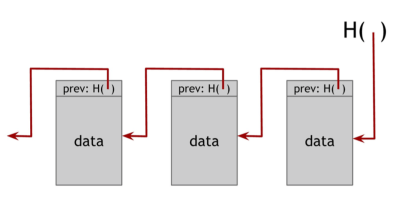
\includegraphics[width=0.8\textwidth]{cadena_de_bloques.png}
     \caption{\textit{Blockchain}: lista enlazada de bloques construida con apuntadores hash. Fuente: \textit{Bitcoin and Cryptocurrency Technologies Book. Princeton University}.\cite{narayanan2016bitcoin}}
    \label{blockchain_linkedlist}
\end{figure}


Desde el punto de vista de negocios, el \textit{blockchain} se  define como una plataforma de tipo \textit{P2P} (por sus siglas en inglés Peer-to-Peer),  mediante la cual los pares pueden intercambiar valores usando transacciones sin la necesidad de un árbitro central de confianza. Esto permite que \textit{blockchain} sea un mecanismo de consenso descentralizado donde ninguna autoridad única está a cargo de la base de datos~\cite{bashir2017mastering}.

Dadas las características y propiedades antes expuestas, la tecnología \textit{blockchain}  se adapta especialmente a escenarios en los que se requiera almacenamiento cronológico de datos, inmutables y cuya confianza no prevalezca en un ente central de control, sino en los participantes involucrados~\cite{wiki:CadenaBloques}.

Dentro de los elementos generales que debería contener cualquier plataforma \textit{blockchain} se encuentran:
\begin{itemize}
    \item Direcciones: las direcciones son identificadores únicos que se utilizan en una transacción dentro del \textit{blockchain} para designar remitentes y destinatarios. Una dirección generalmente es una clave pública. Si bien las direcciones pueden ser reutilizadas por el mismo usuario, las direcciones son únicas. En la práctica, sin embargo, un solo usuario no puede usar la misma dirección nuevamente y generar una nueva para cada transacción. 
    \item Transacción: Una transacción es la unidad fundamental del \textit{blockchain}. Una transacción representa una transferencia de valor de una dirección a otra.
    \item Bloque: Un bloque se compone de varias transacciones y otros elementos como el {\it hash} del bloque anterior ({\it hash pointer}), {\it marca de tiempo} y {\it banderas(bits predefinidos que contienen valores binarios)}.
    \item Red punto-a-punto (P2P): ésta es una topología de red mediante la cual todos los compañeros (nodos de la red) se pueden comunicar entre sí y enviar y recibir mensajes.
    \item {\it Scripting} o lenguaje de programación: los {\it scripts} de transacción son conjuntos de comandos predefinidos para que los nodos transfieran tokens de una dirección a otra y realicen otras funciones. Una característica deseable de los lenguajes utilizados dentro del \textit{blockchain} es que sean “Turing completos”.
    \item Contratos Inteligentes: programas que se ejecutan sobre el \textit{blockchain} y encapsulan la lógica de negocios que se ejecutará cuando se cumplan ciertas condiciones. La función de contrato inteligente no está disponible en todas las cadenas de bloques, pero ahora se está convirtiendo en una característica muy deseable debido a la flexibilidad y la potencia que proporciona a las aplicaciones \textit{blockchain}.
    \item Máquina Virtual: Una máquina virtual permite que el código Turing completo se ejecute en el \textit{blockchain} (como contratos inteligentes), a diferencia  de un {\it script} de transacción que puede estar limitado en su funcionamiento. Las máquinas virtuales no están disponibles en todas las plataformas  \textit{blockchains}; sin embargo, varios plataformas actuales usan máquinas virtuales para ejecutar programas, por ejemplo, Ethereum Virtual Machine (EVM) y Chain Virtual Machine (CVM).
    \item Nodos: Un nodo en una red \textit{blockchain} realiza varias funciones dependiendo del rol que desempeña. Un nodo puede proponer y validar transacciones y realizar operaciones de minería para facilitar el consenso y asegurar la plataforma \textit{blockchain}. Esto se hace siguiendo un protocolo o algoritmos de consenso explicados a continuación. Los nodos también pueden realizar otras funciones, como la verificación simple de pagos (nodos livianos), validadores y muchas otras funciones según el tipo de \textit{blockchain} utilizada y el rol asignado al nodo.
\end{itemize}

\textbf{Características principales}
\begin{itemize}
    \item Consenso Distribuido: El consenso distribuido es el principal soporte de una plataforma \textit{blockchain}. Esto permite que el \textit{blockchain} presente una única versión de la verdad acordada por todas las partes sin el requisito de una autoridad central.
    \item Verificación de transacciones: Todas las transacciones publicadas por los  nodos en el \textit{blockchain} se verifican en base a un conjunto predeterminado de reglas y sólo se seleccionan las transacciones válidas para su inclusión en un bloque.
    \item Transferencia de valores entre pares: El \textit{blockchain} permite la transferencia de valor entre sus usuarios a través de tokens(unidad de valor que una organización crea para gobernar su modelo de negocio). Se puede pensar que los tokens son portadores de valor.
    \item Generación de criptomonedas: En un \textit{blockchain} se  puede generar criptomonedas como un incentivo para sus mineros que validan las transacciones y gastan recursos para asegurar la plataforma. Esta es una función opcional según el tipo de \textit{blockchain} utilizado.
    \item Propiedad intelectual: Es posible vincular un elemento digital o físico al \textit{blockchain} de una manera irrevocable, de modo que no pueda ser reclamado por nadie más; el propietario tiene el control total de su activo y no puede ser gastado doblemente o tener doble propiedad. Esta característica tiene implicaciones de gran alcance, especialmente en la gestión de derechos digitales y en los sistemas electrónicos de efectivo, donde la detección de doble gasto es un requisito clave
    \item Proveedor de seguridad: El \textit{blockchain} se basa en una tecnología criptográfica comprobada que garantiza la integridad y la disponibilidad de los datos. Generalmente, la confidencialidad no se proporciona en primera instancia debido a los requisitos de transparencia(transacciones publicas y visibles para cualquier usuario asociado o no la red blockchain), sin embargo la investigación en esta área ha  madurado y se ha avanzado mucho para obtener confidencialidad y privacidad en las plataformas \textit{blockchain} que necesiten de estas características.
    \item Inmutabilidad: Otra característica clave de \textit{blockchain} es el hecho que los registros que se agregan una vez a la plataforma son inmutables. Aunque teóricamente existe la posibilidad de revertir los cambios, en la práctica se considera casi imposible de lograr, ya que se requiere de una cantidad inaccesible de recursos informáticos, ya que se tendría que accesar a cada uno de los nodos que comparten el registro, alterar cada una de sus decisiones y todo esto en simultaneo, necesitando gran poder de computo para cumplir dicho objetivo.
    \item Unicidad: Esta característica del \textit{blockchain} garantiza que cada transacción sea única y no se haya consumido anteriormente. Esto es especialmente relevante en las plataformas \textit{blockchain} de criptomonedas donde la detección y  evasión  del “doble gasto” son un requisito clave.
\end{itemize}

La Figura~\ref{blockchain_properties} muestra las características de la tecnología \textit{blockchain}.

\begin{figure}[h]
    \centering
    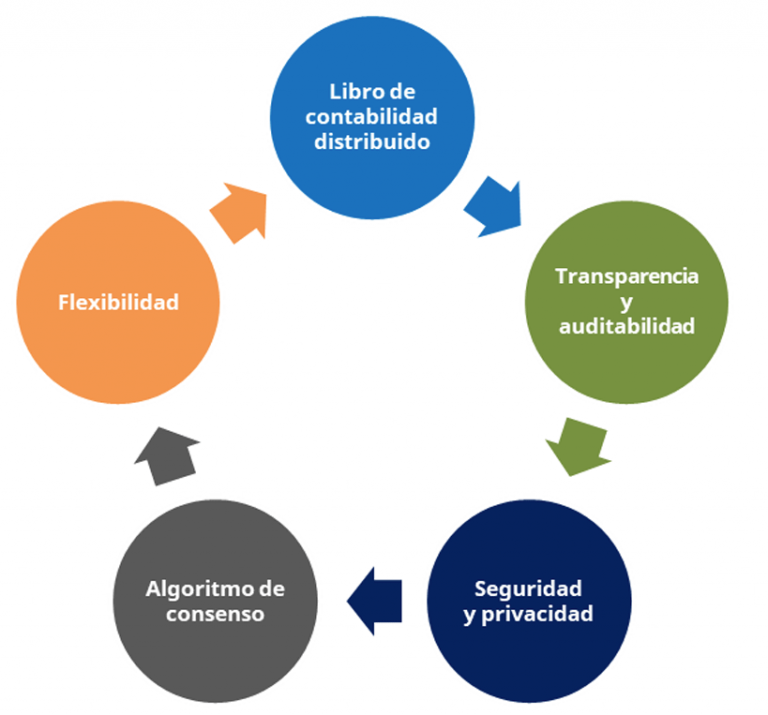
\includegraphics[width=0.5\textwidth]{caracteristicas_blockchain.png}
     \caption{Caracertisticas principales de la tecnologia \textit{blockchain} }
    \label{blockchain_properties}
\end{figure}



\textbf{Tipos de plataformas \textit{blockchain}}:  Basado en la evolución del \textit{blockchain} en los últimos años, esta tecnología se puede dividir en varios tipos con atributos distintos que en muchos casos suelen solaparse:

\begin{itemize}
    \item Públicos:  Estos  tipos de \textit{blockchain}s están abiertos al público y cualquiera puede participar como un nodo en el proceso de toma de decisiones y éstos  pueden o no ser recompensados por su participación. Los registros son propiedad de nadie y están públicamente abiertos para que cualquier persona participe y consulte. Todos los usuarios  mantienen una copia del \textit{blockchain} en sus nodos locales y utilizan un mecanismo de consenso distribuido para tomar una decisión sobre el eventual estado del mismo. Este tipo  también se conocen como libros no permisados.
    \item Privadas: Como su nombre lo indica son privadas y están abiertas sólo a un consorcio o grupo de individuos u organizaciones que han decidido compartir el libro de contabilidad entre ellos.
    \item Semi-privadas: En este tipo de plataformas \textit{blockchain}, una parte del mismo es privada y la otra es pública. La parte privada está controlada por un grupo de individuos, mientras que la parte pública está abierta para la participación de cualquier persona.
    \item Libros contable autorizado: Un libro de contabilidad autorizado es un \textit{blockchain} por el cual los participantes de la red son conocidos y de confianza. Los libros mayores autorizados no necesitan usar un mecanismo de consenso distribuido, en su lugar se puede usar un protocolo de acuerdo para mantener una versión compartida de la verdad sobre el estado de los registros en el \textit{blockchain}. Tampoco es obligatorio que una plataforma \textit{blockchain} autorizada sea privada, ya que puede ser un \textit{blockchain} público, pero con control de acceso regulado.
    \item Libros contable distribuido: Este libro se distribuye entre sus participantes y se extiende a través de múltiples sitios u organizaciones. Este tipo puede ser privado o público. La idea clave es que, a diferencia de muchas otras plataformas \textit{blockchain}, los registros se almacenan de forma contigua en lugar de ordenarse en bloques.
    \item Tokenisadas: Son \textit{blockchain}s estándar que generan criptomonedas como resultado de un proceso de consenso a través de la minería o mediante la distribución inicial. Aquí entra cualquier plataforma relacionada a criptomonedas.
\end{itemize}

\subsection {Sistemas distribuidos}

Primeramente es necesaria la  comprensión de los sistemas distribuidos porque  la tecnología de \textit{blockchain} en su núcleo es un sistema distribuido, específicamente, un sistema distribuido descentralizado.

Los sistemas distribuidos son un paradigma informático mediante el cual dos o más nodos trabajan entre sí en una manera coordinada para lograr un resultado común y está modelada de tal manera que los usuarios finales lo ven como una única plataforma lógica~\cite{bashir2017mastering}.

Se define un nodo como un jugador individual en un sistema distribuido. Todos los nodos son capaces de enviar y recibir mensajes hacia y desde un nodo a otro. Cada nodo posee memoria y procesador propios y se clasifican en tres tipos:  honestos, defectuosos y maliciosos.
%, poseen  memoria y procesador propios. 
Un nodo que puede mostrar un comportamiento arbitrario también se conoce como nodo bizantino. Este comportamiento arbitrario puede ser intencionalmente malicioso, lo cual es perjudicial para el funcionamiento de la red. En general, cualquier comportamiento inesperado de un nodo en la red se puede categorizar como nodo bizantino.

El principal desafío que se presenta en los sistemas distribuidos es la coordinación entre nodos y tolerancia a fallas. Si algunos de los nodos se vuelven defectuosos o se rompen enlaces de red, el sistema distribuido debería ser capaz de  tolerar este tipo de situación y mantener su funcionamiento sin problemas para lograr el resultado deseado.


\subsection{Consenso}
El consenso es un proceso de acuerdo entre nodos desconfiados sobre un estado final de datos. Para lograr el consenso, se pueden usar diferentes algoritmos. En general es fácil llegar a un acuerdo entre dos nodos (por ejemplo en esquemas cliente-servidor) pero cuando múltiples nodos participan en un sistema distribuido y necesitan ponerse de acuerdo en un solo valor, se vuelve complejo lograr dicho consenso. El concepto que define la obtención de consenso entre nodos múltiples se conoce como consenso distribuido (ver Figura~\ref{blockchain_consensus})~\cite{bashir2017mastering}. 

\begin{figure}[h]
    \centering
    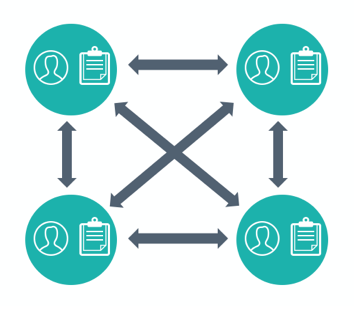
\includegraphics[width=0.4\textwidth]{consenso-nodos.png}
     \caption{Ejemplo de nodos efectuando consenso}
    \label{blockchain_consensus}
\end{figure}

\textbf{Mecanismos de consenso:}  Un mecanismo de consenso es un conjunto de pasos que toman todos, o la mayoría de los nodos, para acordar un estado o valor propuesto~\cite{swanson2015consensus}. Los mecanismos de consenso han pasado recientemente a ser el centro de atención y ganó mucha popularidad con el advenimiento de la primera implementación pública de \textit{blockchain}, la famosa plataforma Bitcoin \cite{nakamoto2008bitcoin}.

Existen cinco requisitos que deben cumplirse para proporcionar los resultados deseados en un mecanismo de consenso:

\begin{itemize}
\item Acuerdo: todos los nodos confiables deciden sobre el mismo valor.
\item Terminación: todos los nodos confiables terminan la ejecución del proceso de consenso y eventualmente llegan a una decisión.
\item Validez: el valor acordado por todos los nodos honestos debe ser el mismo que el valor inicial propuesto por al menos un nodo confiable.
\item Tolerante a fallas: el algoritmo de consenso debería poder ejecutarse en presencia de fallas o nodos maliciosos (nodos bizantinos).
\item Integridad: este es un requisito donde ningún nodo toma la decisión más de una vez. Los nodos toman decisiones solo una vez en un solo ciclo de consenso.
\end{itemize}

Existen varios tipos de mecanismo de consenso, dentro de los dos mas comunes encontramos:
%, dentro de los 2 mas comunes encontramos:
\begin{itemize}
\item Basados en la tolerancia a fallas bizantinas: sin operaciones de cálculo intensivo, como la inversión de hash parcial, este método se basa en un esquema simple de nodos que publican mensajes firmados. Eventualmente, cuando se recibe una cierta cantidad de mensajes, se llega a un acuerdo. Una de las implementaciones más famosas de este tipo, es  el  algoritmo Paxos publicado por Leslie Lamport~\cite{lamport2001paxos}.

\item Basados en líderes: este tipo de mecanismo requiere que los nodos compitan por la lotería de elección de líderes y el nodo que los gana proponga un valor final. Dentro de las implementaciones conocidas de este tipo, destaca el protocolo RAFT publicado por Diego Ongaro y John Ousterhout~\cite{ongaro2015raft}.
\end{itemize}

El concepto de consenso de sistemas distribuidos ha sido incorporado  en la tecnología \textit{blockchain} para proporcionar un medio de aceptación y validación única de la verdad por parte de todos los pares en la red \textit{blockchain}. Dentro de los \textbf{algoritmos de consenso} más importantes que están disponibles hoy o están siendo investigados en el contexto de \textit{blockchain} sobresalen:

\begin{itemize}
\item Prueba de trabajo: este tipo de mecanismo de consenso se basa en la prueba del consumo de recursos computacionales suficientes  antes de proponer un valor para su aceptación por parte de la red. Este mecanismo es utilizado en la plataforma Bitcoin  y otras plataformas \textit{blockchain} asociadas a criptomonedas.
\item Prueba de apuesta: este algoritmo funciona con la idea de que un nodo o usuario tiene una apuesta suficiente en el sistema; por ejemplo, el nodo ha invertido los recursos suficientes  para que cualquier intento de  perjudicar o comprometer a la red concluiria en una perdida de sus propios recursos invertidos. Esta idea fue presentada por el proyecto de Peercoin y se encuentra en etapa de prueba  en el \textit{blockchain} de Ethereum. Otro concepto importante en este tipo de algoritmo es la “edad de la moneda”, que es un derivado desde la cantidad de tiempo y la cantidad de monedas que no se han gastado. En este modelo, las posibilidades de proponer y firmar el siguiente bloque aumentan con la edad de la moneda.
\item Prueba de importancia: esta prueba comparte similitud con la “Prueba de Apuesta” sin embargo este mecanismo no solo se basa en la cantidad de  apuesta que tiene un usuario en el sistema, sino que adicionalmente monitorea el uso y movimiento de los tokens por parte del usuario para establecer un nivel de confianza e importancia. Este mecanismo es utilizado en el proyecto Nemcoin.
\item Prueba de tiempo transcurrido: introducido por Intel, usa un Entorno Confiable de Ejecución (TEE por sus siglas en inglés) para proporcionar aleatoriedad y seguridad en el proceso de elección del líder a través de un tiempo de espera garantizado. Requiere el Intel SGX (Software Guard Extension) procesador para proporcionar la garantía de seguridad\cite{costan2016intel}.
\item Consenso federado o consenso bizantino federado: los nodos en este protocolo mantienen un grupo de pares y compañeros de confianza pública y propaga sólo aquellas transacciones que han sido validadas por la mayoría de los nodos de confianza. Usados en el protocolo de consenso del proyecto Stellar\cite{stellarProject:stellarBasics}
\item Mecanismos basados  en reputación: mecanismo donde un líder es elegido sobre la base de la reputación que ha construido con el tiempo en la red. Esto puede basarse en la votación de otros miembros.
\end{itemize}


%!TEX root = ../thesis.tex

\section{Descentralizacion}  %Title of the First Chapter

La descentralización se ha utilizado en  estrategia, gestión y gobierno durante mucho tiempo. La idea básica consiste en distribuir el control y la autoridad a las periferias en lugar de que una autoridad central tenga el control total de la organización. Esto resulta en varios beneficios para las organizaciones, como una mayor eficiencia, una toma de decisiones más rápida, y una menor carga para la gerencia de bajo y alto nivel~\cite{bashir2017mastering}.

A pesar de no ser un concepto nuevo, la descentralización empieza a tomar gran importancia en el mundo tecnológico, al ser el servicio principal y central brindado por plataformas \textit{blockchain}. Si bien los sistemas descentralizados  y distribuidos tienen mucho en común su principal diferencia radica en que, en los sistemas distribuidos todavía existe una autoridad central que gobierna todo el sistema, mientras que en un sistema descentralizado, no existe tal autoridad. Se podría decir que el \textit{blockchain} es la manera perfecta de proveer una  plataforma que no necesite ningún intermediario o entidad de control, y puede funcionar mediante la interacción de varios participantes o nodos, los cuales definen o validan el estado actual del sistema mediante mecanismos de consenso, específicamente mecanismos de consenso descentralizados que son una verdadera innovación en el paradigma descentralizado. La Figura~\ref{blockchain_descentralziation} compara los tres tipos de redes.

\begin{figure}[h]
    \centering
    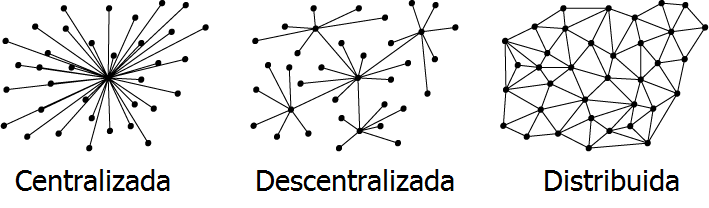
\includegraphics[width=0.8\textwidth]{descentralizacion.png}
     \caption{Diferencia entre redes centralizadas, descentralizadas y distribuidas}
    \label{blockchain_descentralziation}
\end{figure}

Existen dos métodos de descentralización conocidos que pueden ser utilizados:
\begin{itemize}
    \item Desintermediación: El término es bastante común y de uso frecuente en economía e implica la eliminación de intermediarios en una cadena de suministro, o la eliminación de los intermediarios en relación con una transacción o una serie de transacciones~\cite{lin2015infinite}. Un ejemplo de este término aplicado al \textit{blockchain} es la famosa plataforma Bitcoin, en donde se puede  enviar dinero (token) a un conocido, amigo o familiar con solo saber su dirección, eliminando la  necesidad de que una o varias entidades bancarias validen y realicen la transferencia hasta la cuenta destino.
    \item Por competencia:  En este método, un grupo de proveedores de servicios compiten entre sí para ser seleccionados por el sistema para la prestación de servicios. Este paradigma no logra la descentralización completa, pero en cierta medida asegura que un intermediario o proveedor de servicios no esté monopolizando el mismo. En el contexto de tecnología \textit{blockchain}, se puede prever un sistema en el cual los contratos inteligentes pueden elegir un proveedor de datos o nodo candidato externo de una gran lista de proveedores en función de su reputación, puntaje previo, revisiones y calidad del servicio. Esto no dará lugar a una descentralización completa, pero permite que los contratos inteligentes hagan una elección libre en base a los criterios mencionados anteriormente. De esta forma, se crea un entorno de competencia entre los proveedores de servicios, en el que compiten entre sí para convertirse en el proveedor de datos de elección~\cite{bashir2017mastering}.
\end{itemize}

Existe un marco de trabajo que se puede  utilizar para evaluar los requisitos de descentralización de una variedad de elementos en el contexto de la tecnología \textit{blockchain} y que fue propuesto por Arvind Narayanan entre otros~\cite{narayanan2012critical}. El marco básicamente propone cuatro preguntas que se deben responder para generar una idea clara de cómo se puede descentralizar un sistema:
\begin{enumerate}
    \item ¿Qué está siendo descentralizado?
Hace referencia al sistema que se está descentralizando o se quiere descentralizar.
    \item ¿Qué nivel de descentralización se requiere?
Se responde especificando el nivel de descentralización requerido, el cual puede ser aplicando a alguno de los dos métodos discutidos anteriormente: Desintermediacion (descentralizacion total) o Por Competencia (descentralización parcial).
    \item ¿Qué \textit{blockchain} se usa?
Selección de plataforma \textit{blockchain}  adecuada para una aplicación en particular.
    \item ¿Qué mecanismo de seguridad se usa?
Finalmente, es necesario responder a una pregunta clave sobre el mecanismo de seguridad,  en otras palabras cómo se puede garantizar la seguridad de un sistema descentralizado. Un buen ejemplo de esto puede ser la Atomicidad, por el cual la transacción se ejecuta por completo o no se ejecuta en absoluto. El objetivo es asegurar la integridad del sistema.
\end{enumerate}

\subsection{Tipos de organismos descentralizados}
\begin{itemize}
    \item Las organizaciones descentralizadas (DOs, por sus siglas en inglés de {\it Descentralized Organizations})  son programas de software que se ejecutan en una \textit{blockchain} y requiere la interacción constante entre personas o integrantes de la organización para efectuar funciones y operaciones relacionadas a la lógica de negocios. Una vez que una DO, en la forma de un contrato inteligente o un conjunto de contratos inteligentes, se agrega al \textit{blockchain}, el mismo se descentraliza y las partes interactúan entre sí en función del código definido en el software de DO.
    \item Las organización autónoma descentralizada (DAO, por sus siglas en inglés {\it Decentralized Autonomous Organizations})  es básicamente lo mismo que una DO con la diferencia principal que las DAO son autónomos, lo que significa que son completamente automáticos y contienen una lógica artificialmente inteligente, mientras que los DO carecen de esta característica y dependen de los datos humanos para ejecutar la lógica comercial.
    \item Las corporaciones autónomas descentralizadas (DAC, por sus siglas en inglés {\it Decentralized Autonomous	Corporations}) son un concepto similar, pero se consideran un subconjunto de las  DAO. Las definiciones de DAC y DAO se pueden superponer en varios escenarios, sin embargo usualmente difieren en  que los DAO en general se consideran sin fines de lucro, mientras que los DAC pueden ganar dinero a través de acciones ofrecidas a los participantes y mediante el pago de dividendos. Estas corporaciones pueden ejecutar un negocio automáticamente sin intervención humana en función de la lógica programada dentro de ellos.
    \item Las sociedades autónomas descentralizadas (DAS, por sus siglas en inglés {\it Decentralized Autonomous	Societies}) son un concepto mediante el cual sociedades enteras pueden funcionar en un \textit{blockchain} con la ayuda de múltiples contratos inteligentes complejos y una combinación de DAO y aplicaciones descentralizadas (DAPP, por sus siglas en inglés {\it Decentralized	Application}) que funcionan de forma autónoma. Este modelo no significa un enfoque fuera de la ley, ni se basa en una ideología totalmente libertaria; en cambio, muchos servicios que ofrece un gobierno se pueden entregar a través del \textit{blockchain}, como sistemas de tarjetas de identidad del gobierno, emisión de pasaportes y registros de escrituras, matrimonios y nacimientos.
    \item Las aplicaciones descentralizadas (DAPP) son programas de software que pueden ejecutarse en su propia \textit{blockchain}, utilizar otra \textit{blockchain}  o utilizar sólo protocolos de una solución de \textit{blockchain} existente. Todas los DAO, DAC y DO son básicamente aplicaciones descentralizadas que se ejecutan en la parte superior de un \textit{blockchain} en una red punto a punto. Este es el último avance en tecnología con respecto a la descentralización.

\end{itemize}
%!TEX root = ../thesis.tex

\section {Criptografia en Blockchain}  %Title of the First Chapter

%\textcolor{red}{Me parece que el término correcto es crifra, en lugar de encriptar. Verificar.}
%\textcolor{blue} {encriptar cambiado por cifrar en varias partes del parrafo, verificar si es la correcion sugerida. Link de referencia: http://red.computerworld.es/actualidad/cuando-alguien-dice-encriptar-y-quiere-decir-cifrar}

La criptografía es la ciencia encargada del estudio de los algoritmos, protocolos y sistemas que se utilizan para dotar de seguridad a las comunicaciones, a la información y a las entidades que se comunican~\cite{pastor1998criptografia}.

El método en general implica tomar datos sin cifrar, como una pieza de texto, y cifrarlos usando un algoritmo matemático. Esto produce un texto cifrado, una información que es completamente inútil y sin sentido, hasta que se descifra con la ayuda de una clave preestablecida y conocida solamente por el emisor y receptor. Este método  criptográfico se conoce como criptografía de llave simétrica (ver Figura~\ref{blockcain_llavesimetrica}).

\begin{figure}[h]
    \centering
    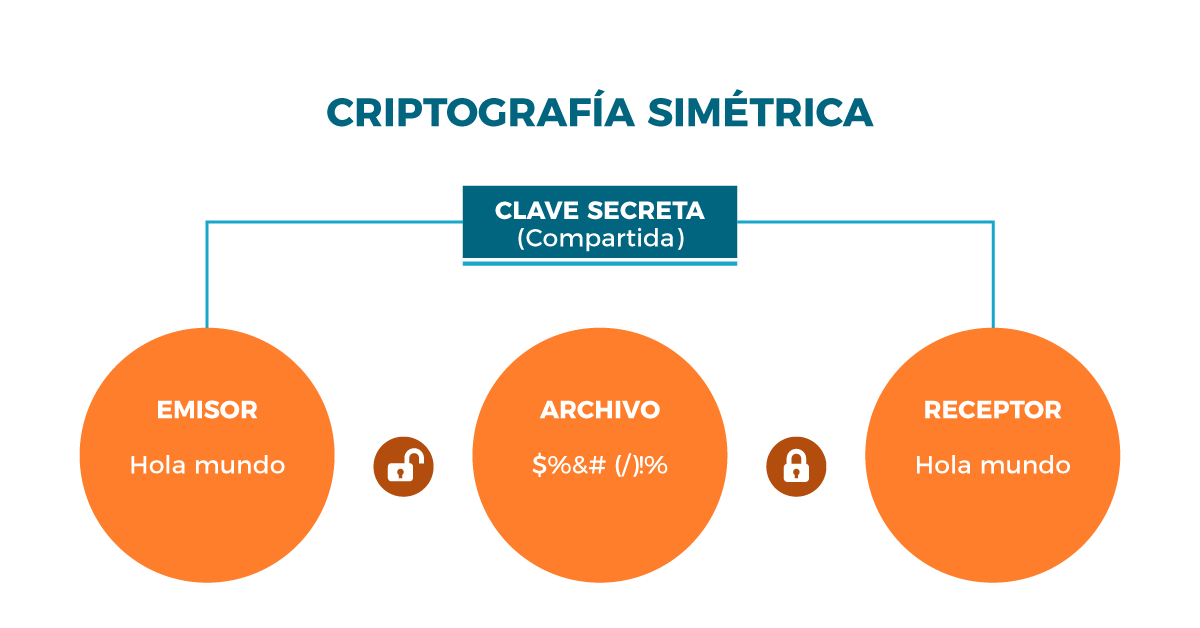
\includegraphics[width=0.7\textwidth]{cripto_simetrica.png}
     \caption{Método criptografico de llave simétrica} 
    \label{blockcain_llavesimetrica}
\end{figure}

La criptografía proporciona varios servicios de seguridad, los cuales son vitales y necesarios en tecnología \textit{blockchain} o cualquier plataforma que haga uso de la misma~\cite{bashir2017mastering}:

\begin{itemize}
    \item \textbf{Confidencialidad} es la garantía de que la información solo está disponible para las entidades autorizadas.
    \item \textbf{Integridad} es la garantía de que la información es modificable sólo por entidades autorizadas.
    \item \textbf{Autenticación} proporciona seguridad sobre la identidad de una entidad o la validez de un mensaje. Hay dos tipos de autenticación:
    La \textbf{autenticación de la entidad} es la garantía de que una entidad está actualmente involucrada y activa en una sesion de comunicacion.
    La \textbf{autenticación de origen de datos}  es la garantía de verificación sobre la fuente de información, esta  implica la integridad de los datos ya que si  una fuente ha sido corroborada, se asegura que los datos no han sido alterados. Diversos métodos, como los códigos de autenticación de mensajes (MAC, por sus siglas en ingles  Message Authentication Code) y las firmas digitales son los más comúnmente utilizados.
    \item \textbf{No repudio}  es la  garantía de que una entidad no puede negar un compromiso o acción previa proporcionando evidencia. El uso de criptografía garantiza que este servicio produce evidencias infalibles e irrefutables  en transacciones electrónicas para que, en caso de disputas, se pueda utilizar como confirmación de una acción.
    \item \textbf{Rendición de Cuentas} es la garantía de que las acciones que afectan la seguridad de la plataforma se pueden rastrear hasta la fuente responsable. Esto generalmente es proporcionado por los mecanismos de registro y auditoría en los sistemas donde se requiere una auditoría detallada debido a la naturaleza del negocio.
\end{itemize}
 
\subsection {Criptografía de llave pública}

A pesar de estar basado en un marco similar, el tipo de criptografía utilizado en \textit{blockchain} es conocida como \textbf{criptografía de llave pública} o \textbf{criptografía asimétrica}, este tipo representa una mejora en la criptografía de llave simétrica estándar, ya que permite que la información se transfiera a través de una llave pública que se puede compartir con cualquier persona~\cite{liskacademy:blockchainCryptographyExplained}.

En la práctica el remitente cifra los datos usando la llave pública del destinatario y luego los transmite a través de la red al receptor. Una vez que llega al receptor, se puede descifrar usando la llave privada del receptor. De esta manera, la llave privada permanece en el lado del receptor y no hay necesidad de compartir llaves para realizar el cifrado y descifrado, que es lo que ocurre en el cifrado simétrico. La Figura~\ref{blockcain_llaveasimetrica} muestra gráficamente este proceso.

Adicionalmente, a través de la criptografía de llave pública se produce una firma digital que garantiza la integridad de los datos que se muestran. Esto se hace combinando la llave privada de un usuario con los datos que desean firmar, a través de un algoritmo matemático.

\begin{figure}[h]
    \centering
    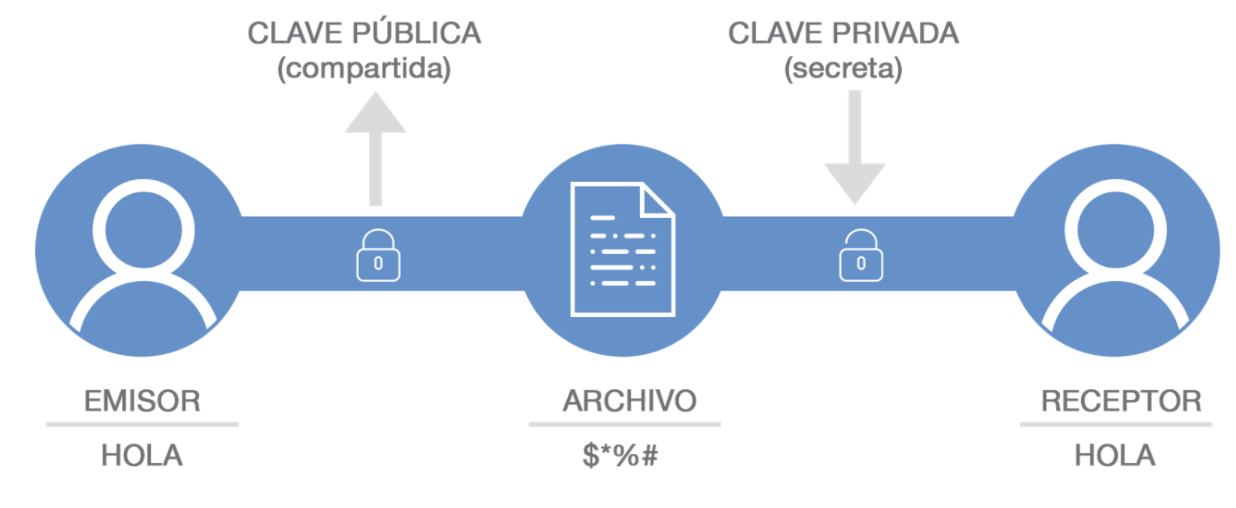
\includegraphics[width=0.7\textwidth]{cripto_asimetrica.png}
     \caption{Método criptográfico de llave asimétrica} 
    \label{blockcain_llaveasimetrica}
\end{figure}

\subsection{Firmas digitales}

Las firmas digitales proporcionan un medio para asociar un mensaje con una entidad desde la cual se originó . Las firmas digitales se usan para proporcionar integridad, autenticación de origen de datos y no repudio.

Dentro de las firmas digitales encontramos 3 propiedades importantes a resaltar, la autenticidad, imposibilidad de force y la no reutilización. Autenticidad significa que las firmas digitales son verificables por una parte receptora. La  imposibilidad de force garantiza que solo el remitente del mensaje pueda usar la funcionalidad de firma con la llave privada y finalmente la no reutilización significa que la firma digital no se puede separar de un mensaje para ser utilizado en otro distinto.

Las firmas digitales son creadas a partir de tres algoritmos cuya finalidad radica en 
hacer absolutamente imposible calcular la llave privada en función de la clave pública o de los datos cifrados y garantizar la autenticidad de una firma basada en el mensaje y la llave privada, verificada a través de la clave pública. A continuación  se describen brevemente los algoritmos:
\begin{itemize}
    \item Un algoritmo de generación de claves, que proporciona una llave privada y pública.
    \item Un algoritmo de firma que combina datos y llave privada para hacer una firma.
    \item Un algoritmo que verifica las firmas y determina si el mensaje es auténtico o no en función del mensaje, la clave pública y la firma.
\end{itemize}

\subsection{Hashing}

Hashing es el proceso de tomar una entrada de cualquier longitud y convertirla en una salida criptográfica fija a través de un algoritmo matemático (Bitcoin usa SHA-256, por ejemplo). Los ejemplos de tales entradas pueden incluir desde un pequeño fragmento de información, como un mensaje hasta un gran caché de información variable, como un bloque de transacciones~\cite{liskacademy:blockchainCryptographyExplained}. La Figura~\ref{blockcain_hashing} ilustra el mecanismo de hashing.

\begin{figure}[h]
    \centering
    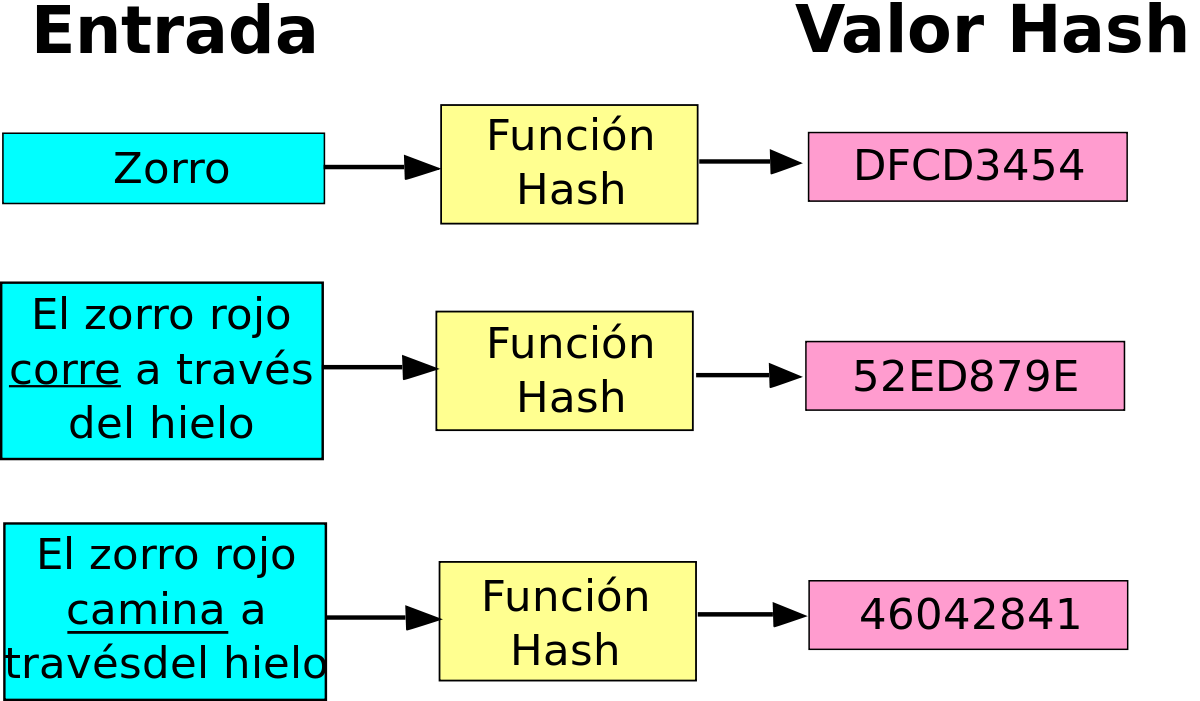
\includegraphics[width=0.6\textwidth]{hashing.png}
     \caption{Ilustración de mecanismo hashing} 
    \label{blockcain_hashing}
\end{figure}

El hashing aumenta drásticamente la seguridad de los datos ya que cualquiera que intente descifrar los datos mirando  el código  hash no podrá calcular la longitud de la información cifrada en función del hash mencionado. Una función de hash criptográfica debe tener varias cualidades cruciales para ser considerada útil:
\begin{itemize}
    \item Imposible producir el mismo valor hash para diferentes entradas.
    \item El mismo mensaje siempre producirá el mismo valor hash.
    \item Rápido en  la  generacion de un hash para cualquier mensaje dado.
    \item Imposible determinar la entrada en función del valor hash.
    \item Incluso el más mínimo cambio a una entrada altera por completo el hash.
\end{itemize}

En \textit{blockchain}, los hashes se usan para representar el estado actual del mundo, o para ser más precisos, el estado del \textit{blockchain}. La entrada representa todo lo que ha sucedido en el \textit{blockchain}, es decir, cada transacción realizada hasta ese punto combinada con los nuevos datos que se agregan.

Como se mencionó, el más mínimo cambio en cualquier parte de la entrada da como resultado un gran cambio en la salida; en esto radica la seguridad irrefutable de la tecnología \textit{blockchain}. Cambiar cualquier registro que haya sucedido previamente en un \textit{blockchain} cambiaría todos los hashes, haciéndolos falsos y obsoletos. Esto se vuelve imposible cuando se toma en cuenta la naturaleza transparente de \textit{blockchain}, ya que estos cambios deberían realizarse a plena vista de toda la red y en todos los nodos que la conforman.

El primer bloque de una cadena de bloques, conocido como bloque de génesis, contiene sus transacciones que, cuando se combinan y validan, producen un hash único. Este hash y todas las transacciones nuevas que se están procesando se usan luego como entrada para crear un nuevo hash que se usa en el siguiente bloque de la cadena. Esto significa que cada bloque se vincula a su bloque anterior a través de su hash, formando una cadena de regreso al bloque de génesis, de ahí el nombre \textit{blockchain}. De esta forma, las transacciones se pueden agregar de forma segura siempre que los nodos de la red estén en consenso sobre cuál debería ser el hash.



\section {Plataformas Blockchain}

En la actualidad, existe una amplia gama de proyectos de código abierto disponibles para la creación de aplicaciones utilizando la tecnología \textit{blockchain}. Aunque la mayor parte de éstos se encuentran relacionados a proyectos de criptomonedas, cada vez más empresas y organizaciones estudian su aplicación en escenarios distintos al del ''dinero digital'', con la finalidad de obtener beneficios (estudiados en secciones anteriores) como por ejemplo, soluciones en cadena de suministros, gestión de propiedad intelectual, administración de procesos de negocio, control de acceso e incluso plataformas de votaciones.

En esta sección se exponen dos de las plataformas más populares y estables en cuanto a documentación, trayectoria, comunidad y soporte se refiere: Ethereum e IBM Hyperledger Fabric. Ambas ofrecen un marco de trabajo (framework) ideal para el desarrollo de aplicaciones basadas en \textit{blockchaion} o DLT (por sus siglas en inglés {\it Distributed Ledger Tecnology}). Asimismo, se presenta una descripción de cada una de las tecnologías y finalmente se definen y comparan sus principales características. 


\subsection{Ethereum}
Ethreum es una red de \textit{blockchain} \textbf{pública} que posee además una criptomoneda denominada \textit{Ether}; también puede ser definida como una plataforma de código abierto que permite a los desarrolladores construir e implementar aplicaciones descentralizadas. Ethereum fue propuesto por Vitalik Buterin a finales de 2013~\cite{wood2014ethereum}, sin embargo fue lanzado oficialmente en julio de 2015. Ha ganado popularidad como plataforma de elección para muchas aplicaciones (DAPP's), así como para la creación y lanzamiento de ICO's (por sus siglas en inglés {\it Initial Coin Offering}). 

Ethereum, cuenta también con la posibilidad de creación de contratos inteligentes que definen reglas y sanciones en torno a un acuerdo, haciendo cumplir obligaciones establecidas en el mismo. En Ethereum, dichos contratos se tratan como {\it scripts} autónomos o aplicaciones descentralizadas (DAPP's) que poseen un estado que se almacena en el \textit{blockchain} para su posterior ejecución. Para su desarrollo, es posible elegir entre varios lenguajes, siendo Solidity el más recomendado. El mecanismo de consenso de Ethereum está basado en la  ''prueba de trabajo'', sin embargo, está previsto cambiarlo por la ''prueba de apuesta'', cual se encuentra en fase de prueba.

Finalmente, Ethereum utiliza una máquina virtual (EVM, por sus siglas en inglés {\it Ethereum Virtual Machine}), es decir, una computadora global distribuida donde se ejecutan todos los contratos inteligentes. Las operaciones efectuadas dentro del EVM, son ejecutadas simultáneamente por cada nodo de la red; por esta razón existe un mecanismo para limitar los recursos utilizados en cada contrato, conocido como \textit{gas}. Cada una las operaciones realizadas tiene un costo medido en gas, y cada unidad de gas consumida por una transacción debe ser pagada en \textit{Ether}.

\subsection{Hyperledger Fabric} 
Hyperledger Fabric es un proyecto avalado e impulsado por \textit{The Linux Foundation} y es mantenido actualmente por IBM~\cite{androulaki2018hyperledger}. Consiste en una infraestructura \textit{blockchain} autorizada de código abierto que proporciona una arquitectura modular y a su vez cuenta con una distinción de roles entre nodos, la cual permite la  ejecución de contratos inteligentes y servicios configurables de consenso y membresía. 

Los contratos inteligentes utilizados en Fabric son llamados ''chaincode'' y pueden estar escritos en Golang, Javascript o Java, y por lo tanto es potencialmente más flexible que un lenguaje cerrado de contratos inteligentes.

Una red Fabric está compuesta por ''pares de nodos'', los cuales son responsables de ejecutar los chaincode, acceder a los datos del \textit{blockchain}, respaldar transacciones e interactuar con aplicaciones. Dichos nodos trabajan de manera autónoma y descentralizada.

Dentro de Hyperledger Fabric, se destaca una herramienta fundamental en la agilización del desarrollo, el \textit{Hyperledger Composer}. Esta herramienta proporciona una interfaz de usuario para la configuración, implementación y prueba de una red de negocios \textit{blockchain}.

\subsection{Diferenciación y Características}

La diferencia fundamental entre Ethereum e Hyperledger se basa en su diseño y público objetivo. Ethereum con su EVM, contratos inteligentes y {\it blockchain} público, está principalmente dirigido a aplicaciones que son de naturaleza distribuida. Por otro lado Hyperledger tiene una arquitectura altamente modular y proporciona mucha flexibilidad en términos de lo que se quiere o no utilizar. Posee varios componentes y herramientas que funcionan de manera \textit{plug-and-play} y está dirigido a organizaciones o empresas que deseen optimizar sus procesos haciendo uso de la tecnología \textit{blockchain}. Por ejemplo, en Ethereum no es posible tener transacciones visibles únicamente para un usuario específico (un requisito frecuente en negocios y organizaciones) a diferencia de Fabric, el cual ofrece ésta y muchas otras herramientas al estar orientado a redes \textit{blockchain} privadas, más específicamente a ''libros contables autorizados''~\cite{blockchaintrainingalliance}.

A continuación se comparan ambas tecnologías en base a 3 aspectos fundamentales: participación de nodos, mecanismos de consenso y arquitectura general.

\subsubsection{Participación de nodos}
Implica que los nodos involucrados en la gestión del \textit{blockchain} pueden contribuir al mismo. En otras palabras, como cada nodo tiene una copia del libro distribuido en una cadena de bloques, importa cómo estos deciden sobre una verdad o estado común, volviendo obligatoria la participación de los nodos en la red.

\noindent
\textbf{Ethereum} \newline
Participación No-Autorizada: se permite la participación de cualquier persona o actor en la red, lo cual tiene sentido al ser un \textit{blockchain} público.

\textbf{Hyperledger Fabric} \newline
Participación Autorizada: los participantes se seleccionan de antemano y sólo éstos tienen acceso a la red, siendo coherente con su naturaleza privada.

\subsubsection{Mecanismos de consenso}

\noindent
\textbf{Ethereum} \newline
En Ethereum, los pares de nodos que participan en la red deben llegar a un consenso para que la transacción pueda ser agregada a la cadena de bloques. Cada nodo debe participar en el logro del consenso, incluso si no ha intervenido en la transacción efectuada. Si un nodo prueba la corrección de una transacción en la red de Ethereum, es recompensado con Ethers. Actualmente, el mecanismo de consenso se establece mediante la minería, la cual está basada en el algoritmo de ''prueba de trabajo''. Sin embargo, tras una actualización reciente conocida como Casper~\cite{buterin2017casper}, se encuentra en fase de prueba el algoritmo de consenso de tipo ''prueba de apuesta'' el  cual se espera sustituya al algoritmo de minería.

\noindent
\textbf{Hyperledger Fabric} \newline 
La definición de consenso en Fabric es diferente. No se limita a la minería basada en ''prueba de trabajo'' o cualquier otro derivado. Dado que éste opera en modo autorizado, hay un control de acceso detallado a fin de mejorar la privacidad.

Aquí, el consenso abarca todo el flujo de transacción desde el principio (propuesta de transacción) hasta el final (inclusión de la transacción dentro del \textit{blockchain}). En este caso, cada nodo asume una función diferente para lograr el consenso, a diferencia de Ethereum, donde todos los nodos tienen el mismo rol.

Los nodos se diferencian según su comportamiento:
\begin{itemize}
    \item Clientes: actúan en nombre de un usuario final; crean y por lo tanto invocan transacciones. Se comunican con  nodos ''pares'' y ''orientadores''.
    \item Pares: Mantienen el \textit{blockchain} y reciben mensajes de actualización ordenados para incluir nuevas transacciones en la plataforma. Los ''endosantes'' son un tipo especial de ''nodos pares'', cuya tarea es respaldar una transacción al verificar si cumplen con las condiciones necesarias y suficientes. (por ejemplo, suministro de firmas requeridas)
    \item Orientadores: proporcionan un canal de comunicación para los nodos clientes y pares, recibiendo y enviando mensajes que contienen la transacción que se puede transmitir.
\end{itemize}

Con Fabric, el algoritmo de consenso empleado es configurable, lo que significa que dependiendo de los requisitos específicos de la aplicación se pueden usar distintos algoritmos. Por ejemplo, para tratar con fallas de replicación aleatorias o maliciosas como se describió anteriormente, se podría usar una variante de los algoritmos de tolerancia a fallas bizantinos.

\subsubsection{Arquitectura general}
\textbf{Ethereum} \newline
El \textit{blockchain} de Ethereum tiene 2 partes principales:

\begin{itemize}
    \item Base de datos: conformada por transacciones que se almacenan en el \textit{blockchain}. Cuando un contrato es ejecutado, por ejemplo, se considera una transacción. Dichas transacciones a pesar de ser públicas (pueden ser vistas y verificadas por todos los participantes) no pueden ser alteradas de manera alguna. Finalmente, para asegurar  que todos los nodos de la red tengan la misma copia de datos, se utiliza el mecanismo de consenso anteriormente descrito, es decir, la ''prueba de trabajo'' para asegurar la plataforma.
    \item Código: en el mundo Ethereum, se escribe el código lógico o de aplicación (contrato inteligente) utilizando un lenguaje denominado Solidity. Posteriormente, se compila \textit{Ethereum Byte Code} y para finalmente implementar ese código de bytes en la plataforma \textit{blockchain}. 
\end{itemize}


Básicamente, el \textit{blockcahin} de Ethereum almacena los datos, el código y lo ejecuta en el EVM. La Figura~\ref{blockchain_ethereum_arquitecture} ilustra  la interacción con la red pública a través del EVM utilizando el paquete de interfaz js \textit{Web3js}

\begin{figure}[H]
    \centering
    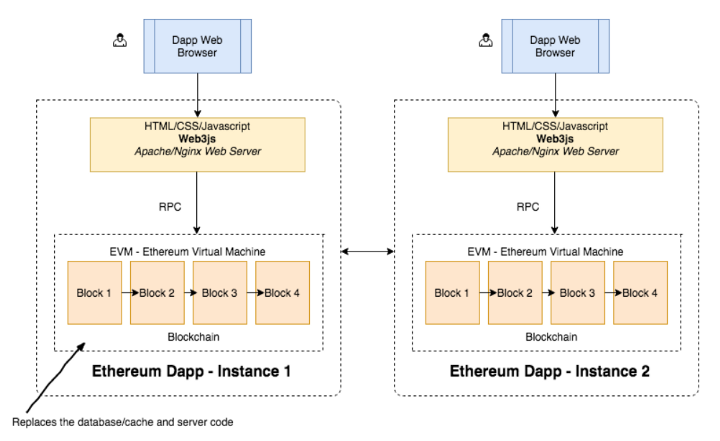
\includegraphics[width=1\textwidth]{ethereum_arquitectura.png}
     \caption{Arquitectura de Ethereum}. 
    \label{blockchain_ethereum_arquitecture}
\end{figure}

\noindent
\textbf{Hyperledger Fabric} \newline
Hyperledger Fabric presenta una arquitectura modular que permite implementaciones integrables de diversas funciones y herramientas. Uno de los elementos fundamentales del Fabric, es su ''protocolo de libro distribuido'', el cual es responsable de la integridad de datos en el \textit{blockchain} y es ejecutado por nodos. Aquí se diferencian 2 tipos de nodos:
\begin{itemize}
    \item Nodo Verificador: es un nodo en la red responsable de ejecutar el consenso, validar las transacciones y mantener el libro contable.
    \item Nodo No-Verificador: es un nodo que funciona como un proxy para conectar clientes (emitir transacciones) con nodos verificadores.
\end{itemize}

Como se mencionó en la sección de mecanismos de consenso, los ''nodos verificadores'' realizan un protocolo a prueba de ''fallas bizantinas'' para ejecutar una máquina de estado distribuido la cual acepta tres tipos de transacciones: implementación, invocación y consulta. La primera, hace referencia a la instalación de un chaincode dentro de un nodo; la segunda ejecuta el chaincode previamente instalado en el nodo (generando posibles cambios de estado) y la última, se refiere a la consulta de estado actual sobre el \textit{blockchain}.

Al estar enfocado en la implementación de libros contables autorizados, Fabric admite la autorización de inscripción y uso de transacciones a través de certificados de clave pública, y la confidencialidad para el chaincode (contratos inteligentes) ejecutados a través de cifrado \textit{in-band}.

En la Figura~\ref{blockchain_fabric_arquitecture}, se visualiza un ejemplo de aplicación de cuidados médicos soportada en Fabric. De lado derecho se aprecia su configuración física, del lado derecho sus componentes lógicos: permisología, nodos, consenso.

\begin{figure}[H]
    \centering
    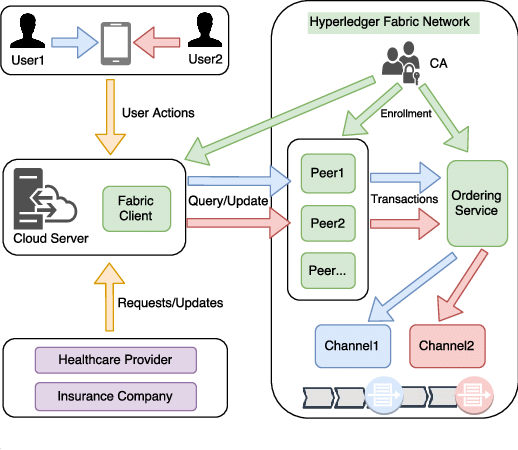
\includegraphics[width=0.8\textwidth]{fabric-arquitectura.png}
     \caption{Arquitectura de Fabric.} 
    \label{blockchain_fabric_arquitecture}
\end{figure}

Finalmente se presenta una tabla comparativa en la Figura ~\ref{blockchain_ethereum_hyperledger}  entre las dos plataformas con las características mas relevantes.

\begin{figure}[H]
    \centering
    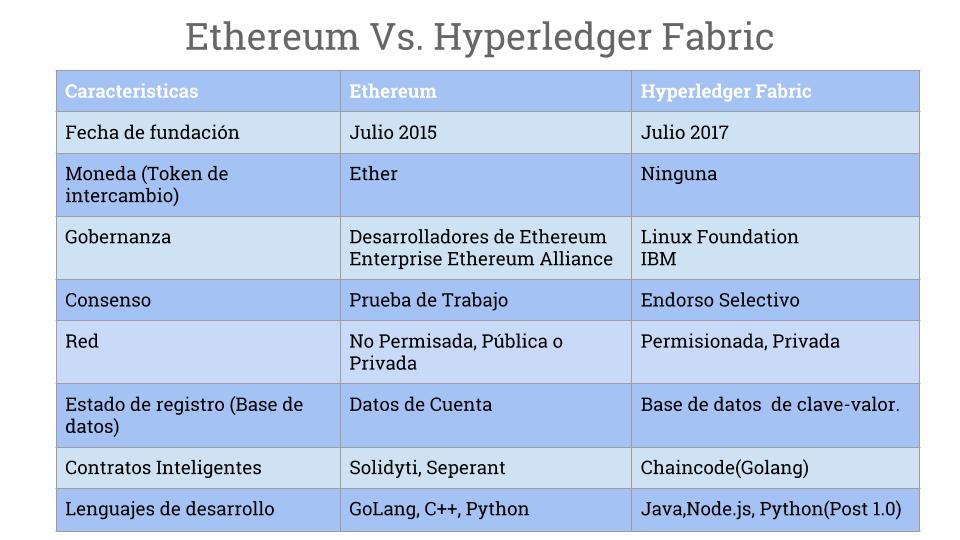
\includegraphics[width=1\textwidth]{Figs/Chapter2/ethereum_vs_hyperledger.jpg}
     \caption{Ethereum Vs. Hyperledger Fabric.} 
    \label{blockchain_ethereum_hyperledger}
\end{figure}


  \graphicspath{ {Figs/Chapter3/} }
 \chapter{Proceso de Creación de un Modelo de red Blockchain}
 
En el presente capítulo, se describe el proceso de creación de un modelo de red \textit{blockchain} utilizando la tecnología Hyperledger IBM, específicamente Hyperledger Composer. Primeramente, se explica la elección de la tecnología; a continuación se presentan conceptos y elementos fundamentales del Hyperledger Composer y finalmente se detallan los pasos necesarios para la creación del modelo de red, siguiendo los lineamientos y conceptos de la tecnología.


\section{Selección de tecnología}
Dado los objetivos planteados en el presente proyecto y haciendo referencia al Capitulo 2, en la Sección 2.4, donde se detallan y comparan las tecnologías existentes, se sugiere el uso  de un \textit{blockchain} de tipo \textbf{privado}, pues éste se adapta mejor a los requerimientos y las necesidades establecidas por la Universidad Simón Bolívar, las cuales ameritan un mayor control sobre el acceso a recursos, roles y permisología asociada a procesos internos de la universidad. Resulta fundamental resaltar que \textit{Hyperledger Fabric} está específicamente diseñado para atender este tipo de escenarios de manera efectiva haciendo uso de su modularidad para adaptarse a los distintos escenarios dentro de las organizaciones. 

\section{Hyperledger Composer y el Modelo de Red Blockchain}

\textit{Hyperledger Composer} es un conjunto de herramientas de colaboración cuya finalidad es construir redes de negocio en \textit{blockchain} y generalmente es utilizado en conjunción de \textit{Hyperledger Fabric}. El Composer permite a los desarrolladores, mediante su abstracción centrada en el negocio, crear contratos inteligentes y aplicaciones \textit{blockchain} de forma rápida y sencilla con la finalidad de dar soluciones robustas a los diferentes problemas sin tener la preocupación inicial del despliegue e instalación de la red \textit{blockchain} a utilizar. Al estar desarrollado con JavaScript, aprovecha las herramientas y librerías modernas, como por ejemplo, node.js, npm y CLI.  

En \textit{Hyperledger Composer}, un modelo de red \textit{blockchain} hace referencia al conjunto de definiciones de los recursos, participantes, elementos y servicios necesarios  dentro de la misma. El modelo de red define el modelo de negocios, la lógica de transacciones (contratos inteligentes) y a su vez delimita las reglas de acceso y permiso lógicas~\cite{dhillon2017hyperledger}.  Dicho modelo de red, está definido en un archivo conocido como \textit{BNA} (por sus siglas en inglés {\it Bussines Network Archive}) y posee la misma extensión para denotarlo (ejemplo, \textit{<nombrearchivo>.bna}). Este archivo es crucial para poder desplegar o instalar una red en \textit{Hyperledger Fabric}. Los elementos específicos del modelo de red \textit{blockchain}, se expondrán en una sección siguiente del presente capítulo.

\section{Proceso de diseño y creación}

El proceso utilizado en la creación de un modelo de red desarrollado en \textit{Hyperledger Composer}, puede ser dividido en 3 fases: planteamiento del problema, diseño del modelo de red e implementación del mismo.

\subsection{Planteamiento del problema y requerimientos} 
Resulta fundamental entender y definir el problema de negocio que requiere solución para posteriormente establecer los requerimientos y necesidades relacionados. 

En \textit{Hyperledger Composer } se definen los siguientes recursos que hacen parte de cualquier modelo de red \textit{blockchain}:
\begin{itemize}
\item Activos: son bienes tangibles o intangibles, servicios o propiedades.
\item Participantes: son miembros de una red de negocios. Éstos pueden poseer activos y enviar transacciones. Cada participante debe contar con un identificador y puede tener otras propiedades asociadas.
\item Transacciones: mecanismo por el cual los participantes interactúan con los activos; también se les conoce como contratos inteligentes o chaincode (en el caso de \textit{Hyperledger}).
\item Reglas y Roles: ésta es la característica principal de cualquier \textit{blockchain} de negocios. Al usar las reglas y roles de acceso, se puede definir quién puede hacer qué y sobre cuáles recursos dentro de la red.
\end{itemize}


\subsection{Diseño y modelado} 
En esta fase se utilizaron una serie de elementos gráficos con la finalidad de representar los distintos recursos de la red previamente definidos. En este fase puede resultar útil la realización de modelos relacionales, diagramas de flujo, actividad, clases o BMPN; en general, cualquier representación que ayude a definir de manera clara las diferentes  interacciones entre los recursos de la red.


\subsection{Implementación y desarrollo}
Desde el punto de vista de desarrollo, el modelo de red \textit{blockchain} está conformado por 3 componentes esenciales:

\textbf{El lenguaje de modelado CTO}: el Composer posee su propio lenguaje de modelado que es utilizado para definir los activos, participantes y transacciones. Estos recursos se definen en un archivo con extensión \textit{.cto} (en honor al  proyecto original denominado \textit{Concert}~\cite{ibmDevWorks}).

Todos los recursos de este archivo están asociados a un \textit{namespace}, el cual funciona como contenedor abstracto base de todas las definiciones de clase comprendidas en la red de negocio. El \textit{namespace} está definido al comienzo del archivo \textit{.cto} de la siguiente manera:

\begin{lstlisting}
namespace org.example.basic
\end{lstlisting}

A continuación se presentan fragmentos de código para cada recurso definido con fines ilustrativos:

\textit{Activo}
\begin{lstlisting}
asset SampleAsset identified by assetId {
  o String assetId
  --> SampleParticipant owner
  o String value
}
\end{lstlisting}
Los activos se diferencian en el lenguaje \textit{CTO} con la palabra \textit{asset} al inicio de su definición y deben poseer al menos un atributo identificador como se observa en el fragmento anterior.

\textit{Participante}
\begin{lstlisting}
participant SampleParticipant identified by participantId {
  o String participantId
  o String firstName
  o String lastName
}
\end{lstlisting}
Los participantes se diferencian en el lenguaje \textit{CTO} con la palabra \textit{participant} al inicio de su definición y deben poseer al menos un atributo identificador como se observa en el fragmento.

\textit{Transaccion}
\begin{lstlisting}
transaction SampleTransaction {
  --> SampleAsset asset
  o String newValue
}
\end{lstlisting}
Las transacciones se diferencian en el lenguaje \textit{CTO} con la palabra \textit{transaction} al inicio de su definición. Pueden tener atributos pero  éstos no son obligatorios.

La letra \textbf{o} sirve para indicar un atributo del recurso, seguido de su tipo y nombre.

El símbolo \textbf{-->} indica la relación con un recurso, seguido del nombre del recurso asociado y su tipo. Esta relaciones son unilaterales.

\textbf{Chaincode o contratos inteligentes}: la lógica de las transacciones definidas en el archivo CTO se implementa gracias a este componente, utilizando el lenguaje de programación Javascript y por consecuencia se encuentran en archivos con extensión \textit{.js} dentro del Composer. A continuación se presenta la implementación lógica de la transacción \textit{SampleTransaction} expuesta en el ejemplo anterior.

\textit{sample.js}
\begin{lstlisting}
/**
 * Sample transaction processor function.
 * @param {org.example.basic.SampleTransaction} tx The sample transaction instance.
 * @transaction
 */
async function sampleTransaction(tx) { 

    // Guarda el valor anterior del activo.
    const oldValue = tx.asset.value;

    // Actualiza el activo con un nuevo valor
    tx.asset.value = tx.newValue;

    // Solicita el registro del activo.
    const assetRegistry = await getAssetRegistry('org.example.basic.SampleAsset');
    // Actualiza el activo en los registros de activos
    await assetRegistry.update(tx.asset);
}
\end{lstlisting}
La siguiente transacción realiza una actualización simple de valor en el activo \textit{SampleAsset} utilizado en los ejemplos del lenguaje de modelado.

Es importante destacar que todas las funciones \textit{.js} deben llevar la cabecera comentada, como se aprecia en el ejemplo, puesto que ésta permite enlazar las funciones lógicas con las transacciones descritas en el modelo CTO.

\textbf{Lista de Control de Accesos}: tanto el control de acceso como la permisología se rigen por un archivo llamado \textit{permissions.acl} (ACL por sus siglas en inglés {\it Access Control Language}). El archivo ACL contiene reglas que le permiten regular el acceso a los recursos de la aplicación \textit{blockchain}. Dichas reglas pueden ser definidas sobre cualquier recurso de la red, es decir, sobre transacciones, activos y participantes. La gramática utilizada para definir estas reglas se puede apreciar en el siguiente ejemplo:

\begin{lstlisting}
rule reglaSimple {
    description: "Descripcion de la regla ACL"
    participant: "org.example.SampleParticipant"
    operation: CREATE, UPDATE
    resource: "org.example.SampleAsset"
    action: ALLOW
}
\end{lstlisting}
\begin{itemize}
    \item El campo \textit{description} es utilizado para colocar una breve descripción del propósito de la regla.
    \item El campo \textit{participant} define la persona o entidad que ha enviado una transacción para su procesamiento. El valor especial \textit{ANY} puede usarse para indicar que no se aplica la comprobación de tipo de participante en la regla.
    \item  El campo \textit{operation} identifica el tipo de operación que rige la regla: \textit{CREATE}, \textit{READ}, \textit{UPDATE}. Adicionalmente, se puede utilizar \textit{ALL} para especificar que la regla rige todas las operaciones compatibles. Alternativamente, es posible utilizar usar una lista separada por comas para especificar que la regla rige un conjunto de operaciones.
    \item  El campo \textit{resource} permite definir cualquier recurso sobre el cual la regla será aplicada.
    \item  El campo \textit{action} identifica la acción de la regla, el cual puede ser \textit{ALLOW} (permitir operaciones asociadas) o \textit{DENY} (denegar operaciones asociadas).
\end{itemize}
 
Una vez desarrollados estos componentes, \textit{Hyperledger Composer} se vale de alguno  de los métodos siguientes para interactuar y probar el modelo de red desarrollado.
\begin{itemize}
    \item El primero, utiliza la herramienta \textbf{Hyperledger Composer Playground} o simplemente \textit{Playground}, que proporciona una interfaz gráfica de usuario para la configuración, implementación y prueba del modelo de red. \textit{Playground} necesita únicamente de un explorador web para empezar a crear, ejecutar y verificar los distintos recursos requeridos en la red de {\it blockchain}.
    
    \item El segundo, a través de una red real desplegada en  \textbf{Hyperledger Fabric} de forma local o en la nube. Este método es de mayor complejidad que el método anterior, ya que requiere una cantidad mayor de herramientas y configuraciones que escapan del alcance de este proyecto. La Figura~\ref{fig: composer-bna} muestra un diagrama explicativo de los componentes del \textit{Composer} y su integracion con \texit{Fabric}.
\end{itemize}

\begin{figure}[h]
\centering
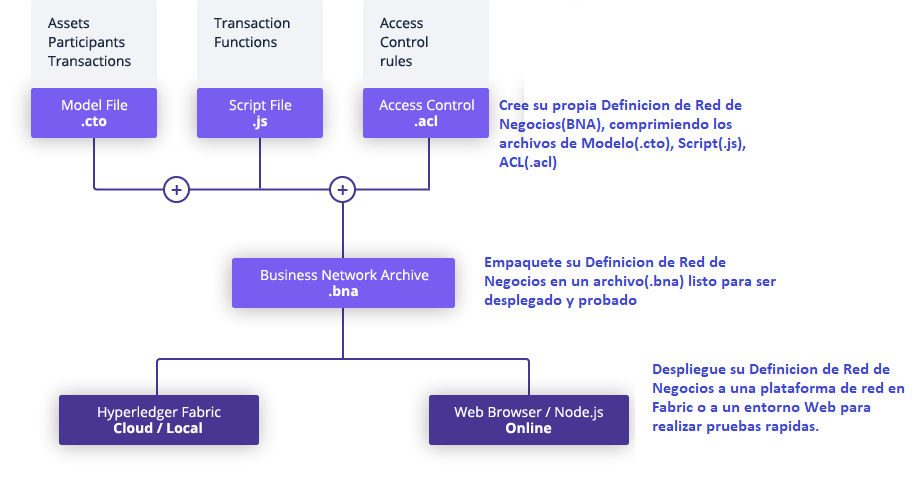
\includegraphics[width=1\textwidth]{composer-playground.png}
\caption[Fabric and Composer]{Diagrama explicativo de componentes del \textit Composer.}
\label{fig: composer-bna}
\end{figure}


 \graphicspath{ {Figs/Chapter4/} }
 
 \chapter{Implementación de un Modelo de red Blockchain}
 
 Con la finalidad de ilustrar la aplicabilidad de la tecnología {\it blockchain} a procesos administrativos universitarios, 
 %cumplir los objetivos trazados, 
 se implementó un modelo de red básico, siguiendo los pasos propuestos en el capítulo anterior. El modelo provee las estructuras necesarias para desarrollar un flujo de trabajo asociado a la transcripción de materias utilizados en universidades. Particularmente, este modelo de red está inspirado en el caso de uso denominado \textit{Creación de Transcripciones} del sistema SIGPAE (Sistema de Gestión de Programas Analíticos de Estudio) de la Universidad Simón Bolívar, que se encuentra actualmente en fase de desarrollo. No obstante, este modelo de red propone funciones y actores adicionales al caso original de SIGPAE, con el propósito de demostrar más ampliamente las características útiles e integrables a este tipo de procesos admiistrativos.
 %presentar una mayor cantidad de características útiles e integrables en el flujo de trabajo del caso de uso anteriormente identificado.
 
 
Para la  implementación del modelo de red se utilizó la herramienta \textit{Hyperledger Composer} versión 0.19.10, usando el lenguaje de programación Javascript versión \textit{ECMAScript5} (para la implementación de la lógica transaccional), el lenguaje de modelado  \textit{Composer CTO} (para definir el modelo de recursos) y el lenguaje  \textit{Compose ACL} (para definir la permisología). Finalmente, para la interacción y prueba de la red se hizo uso de la herramienta \textit{Hyperledger Composer Playground}. 
 
En el capítulo anterior, se describe minuciosamente el proceso de creación del modelo de red \textit{blockchain}. A continuación, se procede a presentar la aplicación de dicho procesos en el diseño e implementación de un modelo de red específico.

\section{Planteamiento del problema y requerimientos}

El proyecto SIGPAE tiene como uno de sus objetivos permitir la transcripción y actualización  de los contenidos programáticos de cada curso o materia que conforman los programas de estudio de la Universidad Simón Bolívar. El proceso consiste en la transcripción digital de un programa de estudio existente(avalado por la coordinacion,departamento o dependencia responsable),la cual es realizada por un transcriptor designado, posteriormente es verificada por un supervisor de transcripción y finalmente es aprobada por DACE(Direccion de Admision y Control de Estudios) una vez comprobada la completitud de la transcripcion. En este contexto, se pretende  crear una plataforma que provea las estructuras necesarias para gestionar lo concerniente al flujo de trabajo relacionado a transcripciones de los contenidos programáticos. 

%El problema identificado, se resume en la necesidad de la creación de una plataforma que provea las estructuras necesarias para gestionar lo concerniente al flujo de trabajo relacionado a transcripciones de programas de estudio. 

Por ende, el modelo de red debe estar diseñado para soportar los siguientes requerimientos:

\begin{itemize}
    \item Permitir la iniciación o creación de una transcripción por parte de los participantes.
    \item Permitir la edición de una transcripción  y actualización de su estado por parte de los participantes.
    \item Manejo de revisiones y observaciones sobre la transcripciones por parte de los participantes.
    \item Gestión de validación y aprobación de la transcripciones por parte de los participantes.
    \item Gestión de accesos y permisos que restrinja las acciones y recursos que pueden ser accedidos por los participantes dentro del flujo de trabajo.
\end{itemize}

Los recursos propuestos para el modelo de red se dividen en:

\textbf{Participantes}
\begin{itemize}
    \item Proponente: da inicio a una transcripción y le asigna un supervisor.
    \item Transcriptor: encargado de realizar la edición de la transcripción.
    \item Supervisor: revisa y valida las transcripciones para su aprobación final.
    \item Auditor: encargado de aprobar transcripciones o enviar observaciones con modificaciones sugeridas para su aprobación.
\end{itemize}

\textbf{Activos} 
\begin{itemize}
    \item Transcripción: elemento o activo del sistema que representa una transcripción de un programa de estudio que aún no se encuentra avalado.
    \item Programa: elemento o activo del sistema que funciona como instancia de un programa de estudio avalado por la USB.
\end{itemize}

\textbf{Transacciones} 
\begin{itemize}
    \item TranscriptorAsignado: asigna un Transcriptor a una \textit{Transcripción}.
    \item SupervisorAsignado: determina la asignación de un supervisor a una Transcripción.
    \item RevisionTranscripcion: ejecuta el envío (guardado) de una revisión con modificaciones sugeridas a una \textit{Transcripcion}. 
    \item ObservacionTranscripcion: ejecuta la operación de enviar (guardar) observaciones a una \textit{Transcripción} necesarias para su aprobación final.
    \item ValidarTranscripcion: efectúa la validación de una \textit{Transcripción}.
    \item AprobarTranscripcion: efectúa la aprobación de una \textit{Transcripción}
\end{itemize}

\section{Diseño y Modelado}
 Se diseñó un diagrama BPMN (por sus siglas en inglés {\it Business Process Model Notation}), que permite identificar el flujo de trabajo sobre una transcripción, las transacciones que se realizan y los participantes involucrados. 
 
 \begin{figure}[H]
    \centering
    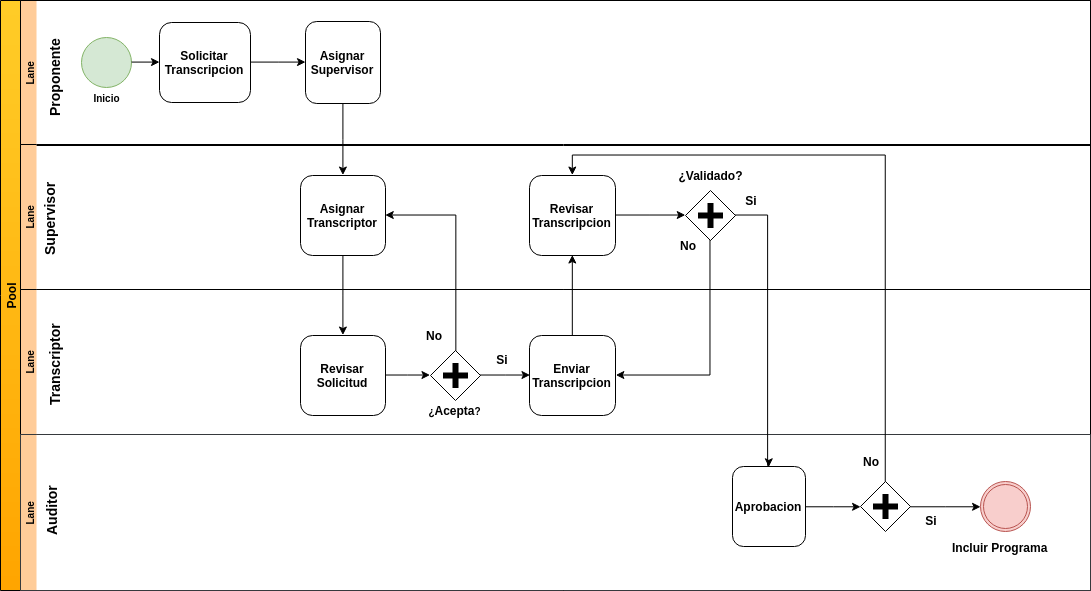
\includegraphics[width=1\textwidth]{flujo_transcripcion.png}
    \caption{Flujo de trabajo de una transcripción}
    \label{flujo_trabajo}
\end{figure}
 

A continuación, se procede a describir los pasos del flujo de trabajo necesarios para la creación de un activo Transcripción, según lo mostrado en la Figura~\ref{flujo_trabajo}.
\begin{enumerate}
    \item El Proponente da inicio al proceso solicitando la creación de una Transcripción.
    \item El Proponente asigna un Supervisor a la Transcripción, una vez iniciado el proceso.
    \item El Supervisor designa un Transcriptor y le envía una solicitud de participación.
     \item Si el Transcriptor acepta la solicitud, se inicia la fase de edición y éste puede empezar a transcribir el programa. De lo contrario, se retorna al paso 3.
     \item El Transcriptor envía la Transcripción para su revisión una vez terminada la edición.
     \item El Supervisor revisa la Transcripción y la valida en caso de estar completa y correcta para iniciar la fase de aprobación. De ser necesaria una modificación, el Supervisor enviará las sugerencias necesarias para su validación y se vuelve al paso 5.
     \item El Auditor realiza una revisión final de la Transcripción. Si ésta cumple todos los requisitos, es aprobada e incluida como programa oficial. De lo contrario, el Auditor procede a enviar observaciones con modificaciones necesarias y se retorna al paso 6.
\end{enumerate}

\section {Implementación y desarrollo}

Finalmente, se presentan los 3 componentes principales que conforman el modelo de red expuestos en el capítulo anterior, que se definen en 3 tipos de archivos. En este capítulo se presenta la estructura del código desarrollado. El código completo se encuentra en el Apéndice A. 
%Por simplicidad el código completo desarrollado se encuentran expuestos en el apartado final de este proyecto y se procede a explicar su estructura.

\subsection{Modelo de Recursos}

%\textcolor{blue}{CORRECION SUGERIDA: Explicación de cuadros de todo el capitulo  }
Este modelo se encuentra descrito en el archivo \textit{programas-academicos.cto} que está incluido en el Apéndice A.
%la sección de \textit{Anexos de Código}. 

A continuación se detallan todos los recursos definidos en este archivo con sus respectiva descripción de atributos y tipos.

\textbf{Participantes}

En el Cuadro \ref{tabla:proponente} se especifica los atributos del  \textit{Proponente}. Se utiliza únicamente el nombre ya que el proponente puede ser una persona particular, una coordinación o dependencia de la universidad interesada en la transcripción de un programa.

\begin{table}[H]
    \captionsetup{justification=raggedleft}
    \caption{\textit{participant Proponente}}
    \centering
    \begin{tabular}{ |c|c|c| }
        \hline
        \textbf{Campo} & \textbf{Tipo} & \textbf{Descripcion} \\ 
             \hline
             participantId & String     & identificador del participante.\\
             nombre        & String     & nombre o alias del participante. \\
             rolAcademico & String & representa la figura académica del participante\\
        \hline
    \end{tabular}
    \label{tabla:proponente}
\end{table}


En el Cuadro \ref{tabla:transcriptor} se presentan los atributos del  Transcriptor el cual debe ser una persona particular, por ejemplo un estudiante, profesor, ayudante académico, entre otros.

\begin{table}[H]
    \caption{\textit{participant Transcriptor}}
    \centering
        \begin{tabular}{ |c|c|c| }
            \hline
            \textbf{Campo} & \textbf{Tipo} & \textbf{Descripción} \\
                 \hline
                 participantId & String     & identificador del participante.\\
                 nombre        & String     & nombre  del participante. \\
                 apellido      & String     & apellido del participante.\\
                 rolAcademico & String & representa la figura académica del participante.\\
                 \hline
        \end{tabular}
    \label{tabla:transcriptor}
\end{table}

En el Cuadro \ref{tabla:supervisor} se presentan los atributos del Supervisor, este debe ser una persona particular y debe tener cierto rango dentro de la comunidad universitaria por ejemplo un profesor.

\begin{table}[H]
    \caption{\textit{participant Supervisor}}
    \centering
     \begin{tabular}{ |c|c|c| }
        \hline
        \textbf{Campo} & \textbf{Tipo} & \textbf{Descripción} \\
             \hline
             participantId & String     & identificador del participante.\\
             nombre        & String     & nombre  del participante. \\
             apellido      & String     & apellido del participante.\\
             rolAcademico & String & representa la figura académica del participante.\\
             \hline
        \end{tabular}
    \label{tabla:supervisor}
\end{table}

En el Cuadro \ref{tabla:auditor} se presentan los atributos del Auditor, el cual debe ser asumido por  una dependencia de la universidad y no una persona particular. Por ejemplo una coordinación, departamento o decanato.

\begin{table}[H]
    \caption{\textit{participant Auditor}}
    \centering
    \begin{tabular}{ |c |c |c| }
        \hline
        \textbf{Campo} & \textbf{Tipo} & \textbf{Descripción} \\
             \hline
             participantId & String     & identificador del participante.\\
             denominacion        & String     & denominación o alias del participante. \\
             rolAcademico & String & representa la figura académica del participante.\\
             \hline
        \end{tabular}
    \label{tabla:auditor}
\end{table}



\textbf{Activos}

El Cuadro \ref{tabla:programa} muestra los atributos del activo Programa del modelo de red.  En la practica los contenidos programaticos (al cual hace referencia este activo) poseen mas atributos sin embargo por motivos de claridad del modelo estos se acotaron a los atributos principales.
\begin{table}[H]
    \caption{\textit{asset Programa}}
    \centering
     \begin{tabular}{ |c| c| c| }
        \hline
        \textbf{Campo} & \textbf{Tipo} & \textbf{Descripción} \\
             \hline    
             recursoId & String     & identificador del programa de estudio.\\
             denominacion & String & denominación o título del programa\\
             codigo & String & código asociado al programa de estudio\\
             contenido & String & contenido programático de la materia\\
             fechaElaboracion & DateTime & denominacion o Fecha de creacion del programa de estudio\\
             \hline
        \end{tabular}
    \label{tabla:programa}
\end{table}

%\textcolor{blue}{CORRECION PROPUESTA: Verificacion de la frase contenidos programaticos}

El activo \textit{Programa} fue incluido con motivos ilustrativos. El modelo de red se concentra en la gestión del activo \textit{Transcripción}.

El Cuadro \ref{tabla:transcripcion} muestra los atributos asociados al activo Transcripción del modelo de red.
Encontramos atributos especiales de tipo \textit{Transaction} o \textit{Transaction List} los cuales permiten asociar las transacciones u operaciones con el activo presentado.

\begin{table}[H]
    \caption{\textit{asset Transcripcion}}
    \centering
    \begin{tabular}{ |c |c |c| }
        \hline
        \textbf{Campo} & \textbf{Tipo} & \textbf{Descripción} \\
             \hline
             recursoId & String     & identificador del programa de estudio.\\
             denominacion & String & denominación o título del programa.\\
             codigo & String & código asociado al programa de estudio.\\
             contenido & String & contenido programático de la materia.\\
             estado & TranscripState & estado actual de una transcripción.\\
             transcriptorAsignado & Transaction &  referencia al transcriptor asociado.\\
             supervisorAsignado & Transaction & referencia al supervisor asociado.\\
             revisionesTranscrip & Transaction List & referencias a revisiones realizadas.\\
             observacionesTranscrip & Transaction List &  referencia a observaciones enviadas.\\
             fechaElaboracion & DateTime & fecha de creación de la propuesta de transcripción\\
             \hline
    \end{tabular}
    \label{tabla:transcripcion}
\end{table}

El campo \textit{estado} puede contener los valores \textit{ESPERA} , \textit{PENDIENTE}, \textit{APROBADO}.


A continuación se presenta en el Cuadro \ref{tabla:transacciones} las distintas transacciones definidas en el modelo con su descripción general.

\begin{table}[H]
    \centering
    \caption{\textit{Lista de Transactions}}
    \begin{tabular}{ |m{10em}|m{10em}|m{5em}| } 
        \hline
        \textbf{Transacción} & \textbf{Descripción} & \textbf {Campos} \\
            \hline
            TranscriptorAsignado &  operación de asignar un transcriptor & -\textit{Relation} transcriptor\\
            \hline
            SupervisorAsignado &  operacion de asignar un supervisor & -\textit{Relation} supervisor\\ 
            \hline
            RevisionTranscripcion &  operación que guarda una revisión en  transcripción & -\textit{String} revisión \\ 
            \hline
            ObservacionTranscripcion &  operación que guarda una observación en transcripción & -\textit{String} observación \\ 
            \hline
            ValidarTranscripcion &  operación que valida una edición  de transcripción y actualiza estado &  \\ 
            \hline
            AprobarTranscripcion & operación que aprueba una transcripción y actualiza estado &  \\ 
            \hline
    \end{tabular}
    \label{tabla:transacciones}
\end{table}

Todas las transacciones poseen una relación a Transcripción lo que permite  agregarlas dentro del registro del activo.

El campo \textit{Relation} en las transacciones \textit{TranscriptorAsignado} y \textit{SupervisorAsignado} permiten asociar al participante objetivo dentro del registro de la transacción.

El campo \textit{String} en las transacciones \textit{RevisionTranscripcion} y \textit{ObservacionTranscrip} permite guardar la revisión u observación dentro del registro de la transacción.

\subsection{Chaincodes o Lógica de transacciones}
La lógica de transacciones del modelo de red se encuentra definida   en funciones de Javascript, descritas en el archivo \textit{transcripcion.js} mostrado en detalle en el Apéndice A.
%incluido en la seccion de Anexos de Codigo. 

Se  presentan a continuación las funciones asociadas a las transacciones en el Cuadro \ref{tabla:chaincodes}.

 \begin{table}[H]
     \centering
          \caption{Chaincodes}
     \begin{tabular}{|m{10em}|m{22em}|}
         \hline
         Función & Descripción  \\
         \hline
         transcriptorAsignado & Actualiza el  campo \textit{transcriptorAsignado} de una transcripción con el transcriptor seleccionado \\
         \hline
         supervisorAsignado & Actualiza el campo \textit{transcriptorAsignado} de una transcripción con el supervisor seleccionado\\
         \hline
         revisionTranscripcion & Agrega una revisión en la lista asociada al  campo \textit{revisionesTranscripcion} de una transcripción \\
         \hline
         observacionTranscripcion & Agrega una observación a la lista asociada al campo \textit{observacionesTranscripcion} \\
         \hline
         validarTranscripcion & Actualiza el campo \textit{estado} de una transcripción con el valor \textit {PENDIENTE} indicando que la transcripción esta pendiente de aprobación\\
          \hline
         aprobarTranscripcion & Actualiza el campo \textit{estado} de una transcripción con el valor \textit{APROBADA} indicando que la transcripción fue aprobada y está pendiente su inclusión como programa de estudio.\\
         \hline
     \end{tabular}
     \label{tabla:chaincodes}
 \end{table}

No es necesario que las funciones tengan el mismo nombre que la transacciones encontradas en el archivo \textit{CTO}, sin embargo se recomienda utilizar esta práctica para mayor claridad.


\subsection{Lista de control de accesos}
Las reglas de  permisologia y accesos asociados a los recursos del modelo de red se describen en el archivo \textit{permission.acl} incluido en el Apéndice A.
%la seccion de Anexos de Codigo.

Se utilizó la siguiente nomenclatura para  nombrar las diferentes reglas del archivo \textbf{rule Participante\_Permisos\_Recurso}

Este patrón permite identificar y entender rápidamente el cometido de la regla. Por ejemplo, la regla:

\centerline{ \textit{rule Proponente\_RC\_Transcripcion}\{\} }   

Describe que el  participante  \textit{Proponente} tiene permisos  \textit{READ} y \textit{CREATE} (leer y crear), sobre el activo \textit{Transcripción}. 

En  los cuadros \ref{tabla:reglas_activos} y \ref{tabla:reglas_transacciones} se presentan los permisos sobre los activos y transacciones del modelo de red. En el primero se describen los accesos a los activos del modelo de red, y las acciones permitidas sobre este, quien puede ver, crear o realizar modificaciones sobre el activo mencionado. El segundo cuadro se exponen los participantes habilitados para la ejecución de las distintas transacciones del modelo.
 
\begin{table}[H]
    \centering
    \caption{Reglas definidas para los Activos del modelo de red}
    \begin{tabular}{|m{6em}|m{6em}|m{6em}|m{14em}|}
        \hline
            \multicolumn{4}{|c|}{Reglas sobre Activos}\\
        \hline
            \textbf{Activo} & \textbf{Participante(s)} & \textbf{Permiso(s)} & \textbf{Restricción}  \\
        \hline
            \multirow{2}{10em}{Transcripción} & Proponente & CREAR LEER & solo el proponente puede crear (iniciar) una transcripción \\
            & Transcriptor Supervisor Auditor & MODIFICAR LEER & todos menos el proponente puede modificar una transcripción.\\
        \hline
            Programa & Todos & LEER & todos los participantes pueden leer y visualizar un programa\\
        \hline
    \end{tabular}
    \label{tabla:reglas_activos}
\end{table}

\begin{table}[H]
    \centering
    \caption{Reglas definidas para las Transacciones del modelo de red}
    \begin{tabular}{|m{10em}|m{6em}|m{14em}|}
    \hline
        \multicolumn{3}{|c|}{Reglas sobre Transacciones}\\
    \hline
        \textbf{Transacción} & \textbf{Participante} & \textbf{Restricción}  \\
    \hline
         TranscriptorAsignado & Supervisor & sólo el supervisor puede asignar un transcriptor \\
         \hline
         SupervisorAsignado & Proponente & solo el proponente puede asignar un supervisor\\
         \hline
         RevisionTranscripcion & Auditor & solo el auditor puede hacer observaciones sobre una transcripción \\
         \hline
         ObservacionTranscripcion & Auditor & sólo el auditor puede hacer observaciones sobre una transcripción \\
         \hline
         ValidarTranscripcion & Supervisor& solo el supervisor puede validar un transcripción\\
         \hline
         AprobarTranscripcion & Auditor & solo el auditor puede aprobar una transcripción\\
    \hline
    \end{tabular}
    \label{tabla:reglas_transacciones}
\end{table}

\section{Interacción y prueba del modelo de red}

Para poder interactuar y probar el modelo de red, se utilizó la herramienta \textit{Composer Playground}. Como se definió en el capitulo anterior, esta herramienta provee una interfaz gráfica que permite probar el modelo de red, específicamente revisar los registros de recursos, probar transacciones e incluso implementar código que se ejecuta de manera inmediata. \textit{Composer Playground} puede ser utilizado con  una instalación local o a través de su aplicación en línea~\cite{composerPlayground}.

\textit{Hyperledger Composer} solo necesita los 3 archivos descritos en las secciones anteriores \textit{programas-academicos.cto}, \textit{transcripcion.js} y \text{permission.acl} para iniciar el modelo de red cómo se expone a continuación:

Se presenta la interfaz gráfica \textit{Playground}. La interfaz es bastante intuitiva y fácil de manejar, se concentra en la prueba de transacciones y verificaciones de registros definidos en el modelo de red. En la figura \ref{fig: playground-presentation} se aprecia una primera impresión de la interfaz donde es posible ver el histórico de transacciones realizadas hasta el momento.

\begin{figure}[H]
\centering
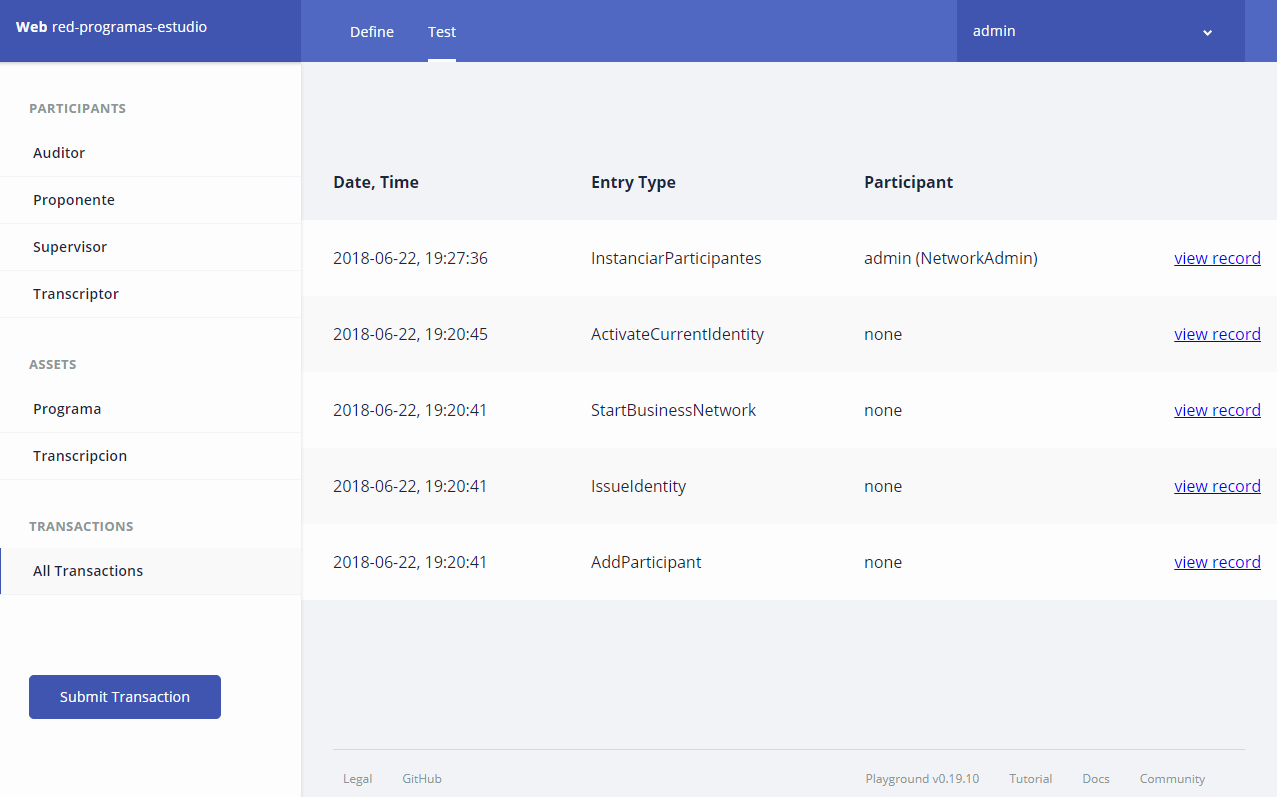
\includegraphics[width=1\textwidth]{playground1.png}
\caption[Interface Playground]{Interfaz gráfica  de Playground.}
\label{fig: playground-presentation}
\end{figure}

La funcionalidad principal del playground se resume en 2 pestañas principales, \textit{Test} y \textit{Define}, ubicadas en la esquina superior izquierda de la interfaz y se muestran en la figura \ref{fig: playground-tabs}. La pestaña \textit{Test} se utiliza para consultar registros, probar transacciones y verificar el  histórico de transacciones realizadas dentro de la red. La pestaña \textit{Define} se utiliza para definir y desarrollar los 3 componentes del modelo de red nombrados a lo largo de todo el capitulo.

\begin{figure}[h]
\centering
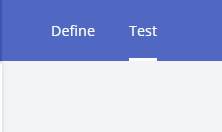
\includegraphics[width=0.5\textwidth]{playground7.png}
\caption[Tabs Playground]{Pestañas de Playground }
\label{fig: playground-tabs}
\end{figure}

El panel izquierdo de la pestaña \textit{Test}  permite visualizar los recursos de la red (\textit{Participantes}, \textit{Activos}, e histórico de \textit{Transacciones}, haciendo click en cualquier de los elementos expuestos en la figura \ref{fig: playground-test-sidebar})
\begin{figure}[H]
\centering
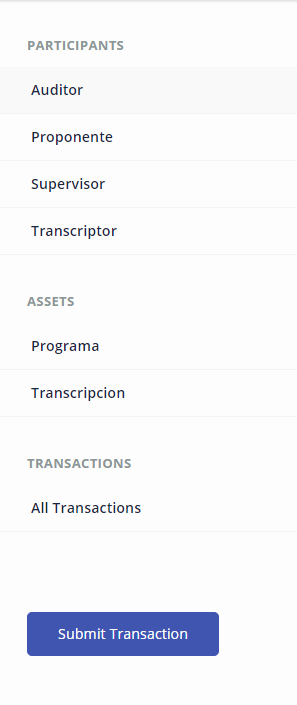
\includegraphics[height=0.5\textheight]{playground2.png}
\caption[Test Sidebar Playground]{Panel lateral de la pestaña \textit{Test} en \textit{Playground} }
\label{fig: playground-test-sidebar}
\end{figure}

En la sección principal de la pestaña \textit{Test},se puede visualizar los diferentes recursos agregados a la red. En la figura \ref{fig: playground-test-principal} se muestran los registros de \textit{Transcripción} \textit{A\_TRANS001} y \textit{A\_TRANS002} cada uno representa la transcripcion de un programa de estudio de la cadena de matemáticas (\textit{Matematicas I }y \textit{Matematicas II} respectivamente).

\begin{figure}[h]
\centering
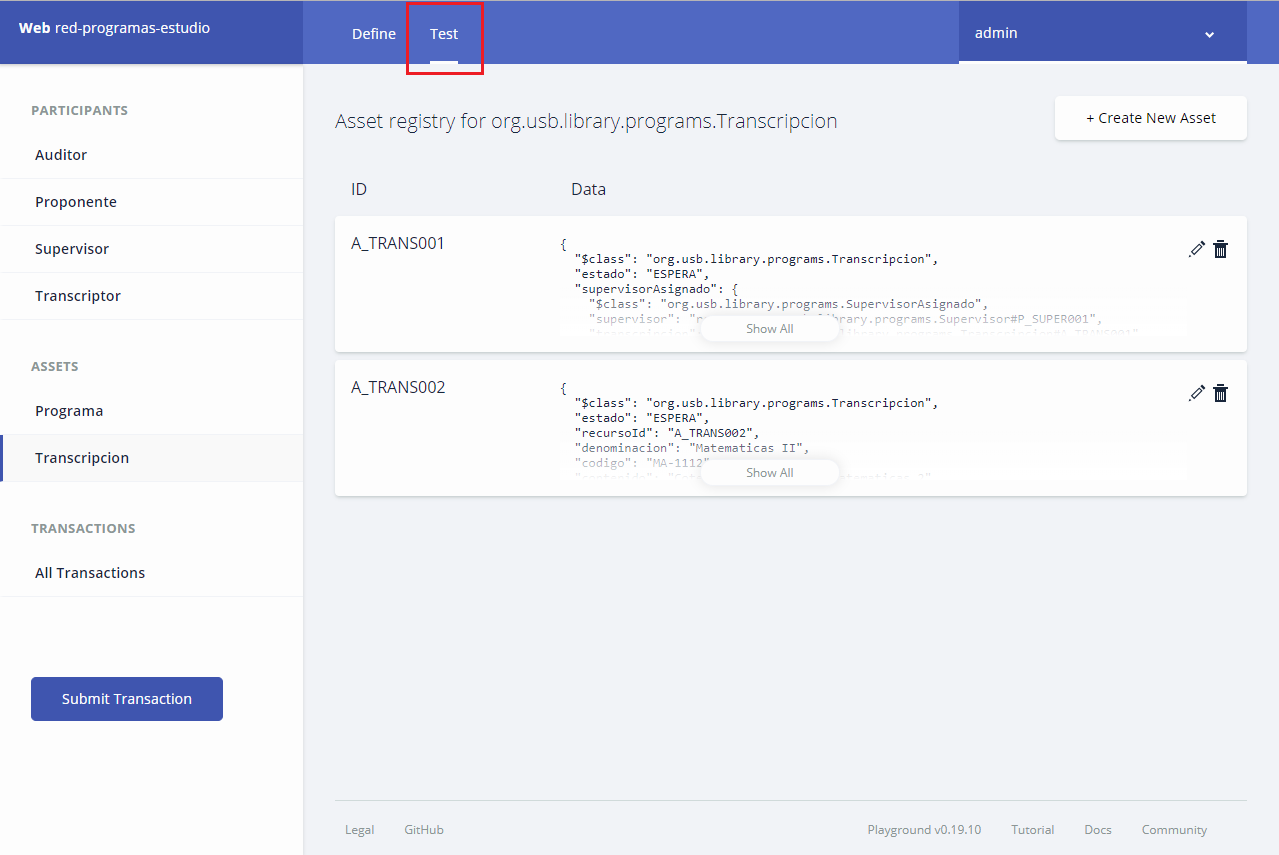
\includegraphics[width=1\textwidth]{playground3.png}
\caption[Test Principal Playground]{Seccion principal de la pestaña \textit{Test} }
\label{fig: playground-test-principal}
\end{figure}

En la figura \ref{fig: playground-test-register} se aprecia un ejemplo de la transcripción en proceso del programa de estudios de \textit{Matemáticas I} (código de materia \textit MA-1111)

\begin{figure}[H]
\centering
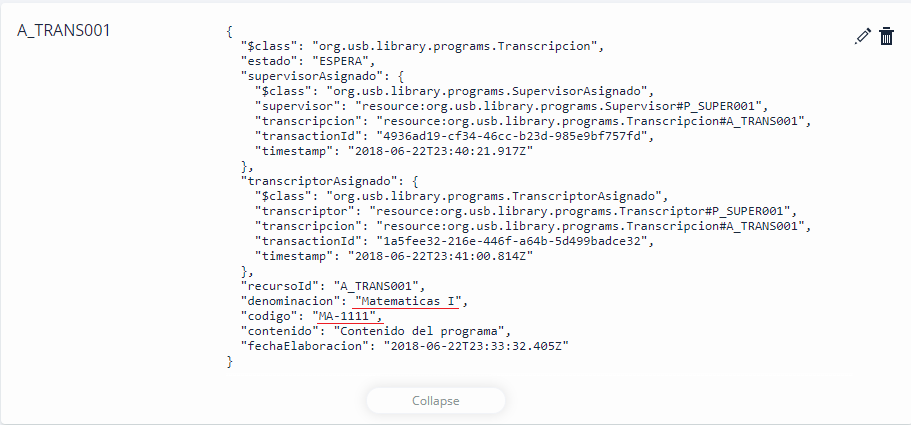
\includegraphics[width=1\textwidth]{playground4.png}
\caption[Test Register Playground]{Vista detalla de un registro de \textit Transcripcion.}
\label{fig: playground-test-register}
\end{figure}

Para la ejecución y prueba de transacciones se utiliza la opción \textit{Submit Transaction} encontrada al final del panel izquierdo de la pestaña \textit{Test} como se muestra en la figura \ref{fig: playground-test-transaction} que también  muestra  las transacciones del modelo descritas en el Capítulo 3.

\begin{figure}[h]
\centering
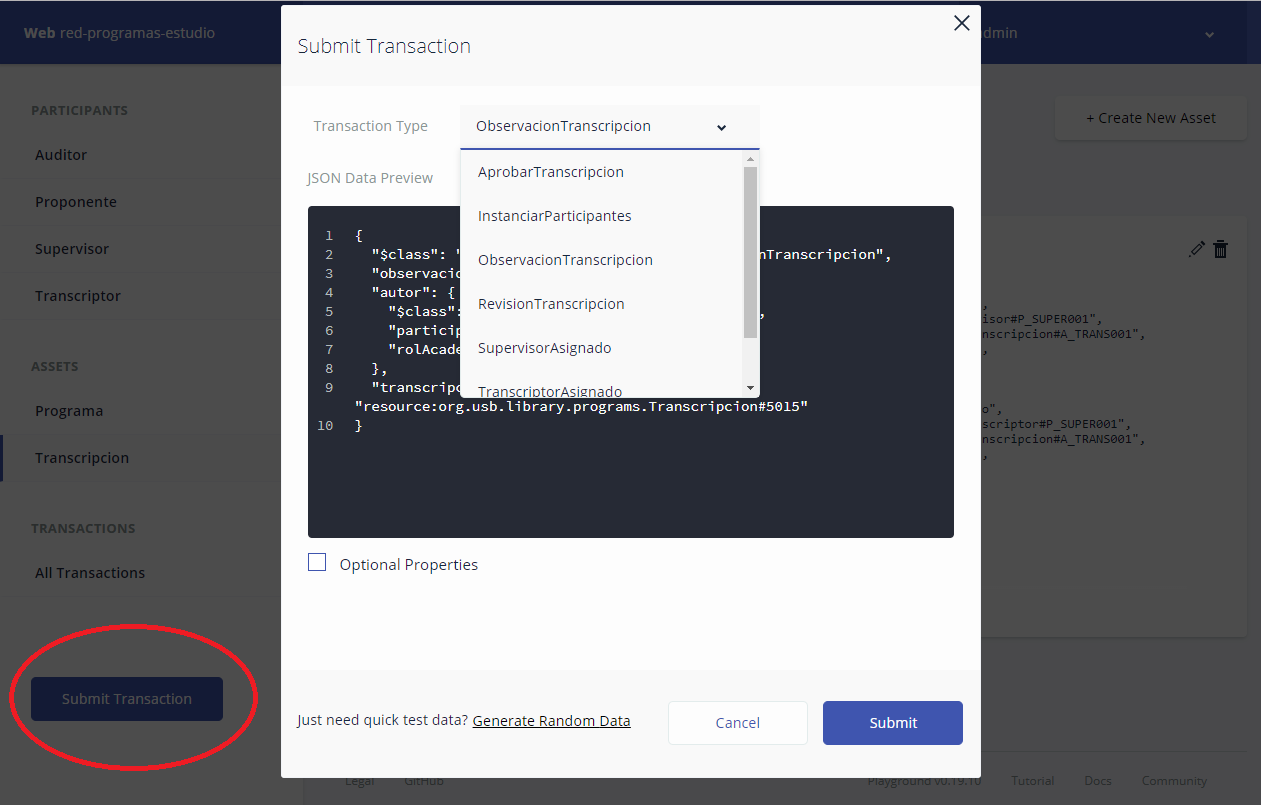
\includegraphics[width=1\textwidth]{playground5.png}
\caption[Test Transaction Playground]{Ventana de prueba y ejecución de transacciones o chaincodes}
\label{fig: playground-test-transaction}
\end{figure}

La pestaña \textit{Define}  permite crear y codificar los archivos necesarios para iniciar el modelo de red. En la figura \ref{fig: playground-define-principal} se expone el editor de texto que provee \textit{Playground} para el desarrollo y visualización de archivos.

\begin{figure}[h]
\centering
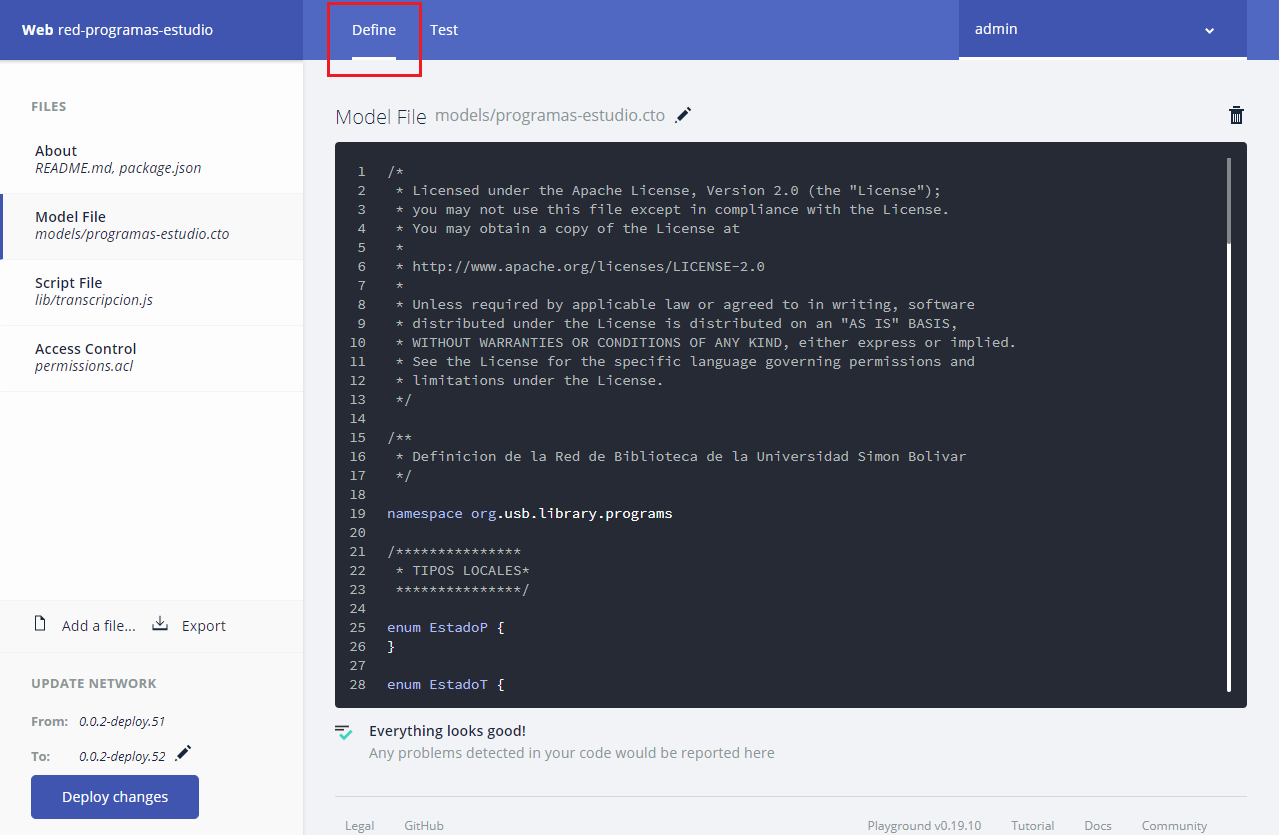
\includegraphics[width=1\textwidth]{playground6.png}
\caption[Define Principal Playground]{Pestaña \textit{Define} vista general.}
\label{fig: playground-define-principal}
\end{figure}

En el panel izquierdo de la pestaña \textit{Define} podemos encontrar los archivos  necesarios del modelo de red. En la figura \ref{fig: playground-define-sidebar} se aprecian los archivos descritos en el capitulo 4: \textit{programas-estudio.cto}, \textit{transcripcion.js}, \textit{permissions.acl}. Todos pueden ser vistos y editados a traves del editor de texto dinamico mencionado anteriormente.
\begin{figure}[H]
\centering
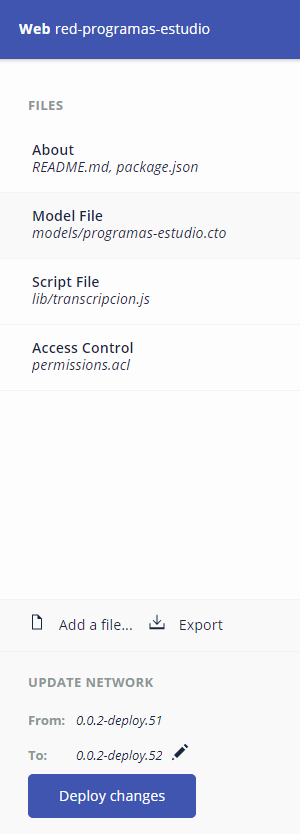
\includegraphics[height=0.6\textheight]{playground8.png}
\caption[Define Sidebar Playground]{Panel lateral de la pestaña \textit{Define}}
\label{fig: playground-define-sidebar}
\end{figure}

Como ilustra la figura \ref{fig: playground-define-export}, las opciones al final del panel permiten agregar archivos locales, desplegar o guardar los cambios y principalmente exportar (crear) el archivo \textit{BNA} necesario para levantar una red blockchain real en \textit{Hyperledger Fabric} como se explica en el capitulo 3.
\begin{figure}[H]
\centering
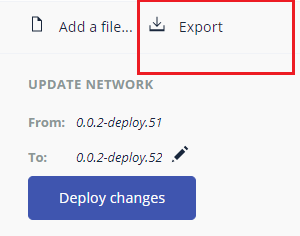
\includegraphics[width=0.3\textwidth]{playground9.png}
\caption[Define Export Playground]{Opcion \textit{Export} al final del panel lateral}
\label{fig: playground-define-export}
\end{figure}


%!TEX root = ../thesis.tex

\chapter{Conclusiones y recomendaciones}
\label{capitulo5}
En la actualidad, la implantación de sistemas basados en \textit{blockchain}, a  excepción de aquellos proyectos financieros destinados a criptomonedas, es escasa. No obstante, existen organizaciones de diverso índole que pueden beneficiarse de las oportunidades que presenta esta tecnología. Seguridad, transparencia y confianza son características que pueden mejorar e incluso escalar distintos procesos dentro de organizaciones, empresas y academias.

Durante la realización del presente trabajo, se abordaron conceptos principales tanto teóricos como prácticos que definen a la tecnología \textit{blockchain}, cuáles son sus beneficios y tipos de uso. Alejada de la visión financiera tradicional (criptomonedas), la intención del autor fue destacar la utilidad y beneficios de la cadena de bloques en otros sectores y rubros, tal como la implementación de una solución \textit{blockchain} orientada a soportar y mejorar procesos administrativos dentro de la Universidad Simón Bolívar.


El modelo de red \textit{blockchain} desarrollado está inspirado en la funcionalidad de gestión de transcripciones del sistema \textit{SIGPAE}. Fue diseñado e implementado con fines exploratorios e ilustrativos, buscando exponer las diferentes características que la tecnología \textit{blockchain Hyperledger}  puede ser usada de manera total o parcial por un sistema interno de la Universidad Simón Bolívar. 

A pesar de su breve trayectoria, la tecnología \textit{blockchain} ha demostrado ser efectiva cumpliendo con todas las características expuestas a lo largo de este trabajo. Por otro lado, la existencia de diversos proyectos de criptomonedas (implementaciones utilizadas en el mundo real) que en su gran mayoría han garantizado inmutabilidad, transparencia y confiabilidad, genera una razón de peso al momento de pensar en la tecnología \textit{blockchain} como posible solución tecnológica, o mejor aún como posible componente de una solución donde se integren otros tipos de tecnología tal como inteligencia artificial o internet de las cosas, sólo por nombrar algunas.

Resulta de gran importancia recalcar que el modelo de red desarrollado puede ser perfectamente ampliado, refactorizado o simplemente servir de referencia para realizar un modelo más acorde y alineado con los requerimientos de los diferentes procesos del sistema \textit{SIGPAE}. 

Durante el desarrollo del proyecto se realizo una implementación de una red local de prueba utilizando la plataforma Hyperledger Fabric, en una sola computadora que utilizando contenedores \textit{Docker}() logra levantar 2 nodos para dicha prueba. Sin embargo, dada la complejidad  de esta herramienta, no fue expuesta  en este proyecto con el objetivo de  respetar la extensión máxima requerida en proyectos de grado de la Universidad Simon Bolivar.

Por tal motivo  se presentan una serie de consideraciones de importancia para estudios e investigaciones posteriores a fin de cumplir con la secuencia lógica y pretendiendo ser un valioso aporte para futuros trabajos de investigación.


\begin{itemize}
    \item En primer lugar, se sugiere la instalación de una red local o en su defecto su simulacion con ayuda de contenedores docker con el marco de trabajo \textit{Hyperledger Fabric}, para poder observar y verificar la integración del modelo red encontrado en el repositorio ~\cite{github:usb-library-network} con las funcionalidades principales de la tecnología \textit{blockchain}, nodos, mecanismos de consenso y criptografía.
    
    Se sugiere utilizar el modelo de red desarrollado en este proyecto, el cual se encuentra publico y disponible en el siguiente repositorio de github.
    
    Adicionalmente se aconseja la consulta del siguiente recurso que será de gran de utilidad para este fin:  \textit{Instalación y prueba de un red \textit{blockchain} en Fabric}~\cite{localFabric}.
    
    \item Seguidamente, se sugiere el despliegue de una red \text{Fabric} en un servidor propio o algún proveedor de servicios en la nube, con la finalidad de poder observar el comportamiento de la red \textit{blockchain} en un escenario real. En la documentación suministrada por IBM se encuentran recursos y guías que facilitan este objetivo: \textit{Despliegue de una red Fabric en una organización}~\cite{organizationFabric}
    
    \item Finalmente, se sugiere el uso de la herramienta de {\it testing} \textit{Cucumber}, para probar toda la lógica de transacciones y permisologías asociadas a la red implementada. Esta herramienta es recomendada por desarrolladores de \textit{IBM Hyperledeger}, lo que permite asegurar el cumplimiento de criterios de calidad sobre la plataforma \textit{blockchain} desarrollada~\cite{testingCucumber}.
.
\end{itemize}




%\include{code/code}
%\include{Chapter3/chapter3}
%\include{Chapter2/chapter2}
%\include{Chapter4/chapter4}
%\include{Chapter5/chapter5}
%\include{Chapter6/chapter6}
%\include{Chapter7/chapter7}



% ********************************** Back Matter *******************************
% Backmatter should be commented out, if you are using appendices after References
%\backmatter

% ********************************** Bibliography ******************************
\begin{spacing}{0.9}

% To use the conventional natbib style referencing
% Bibliography style previews: http://nodonn.tipido.net/bibstyle.php
% Reference styles: http://sites.stat.psu.edu/~surajit/present/bib.htm

%\bibliographystyle{apalike}
%\bibliographystyle{unsrt} % Use for unsorted references
%\bibliographystyle{plainnat} % use this to have URLs listed in References
\bibliographystyle{IEEEtran}
%\bibliographystyle{unsrt}
\cleardoublepage
\bibliography{References/references} % Path to your References.bib file


% If you would like to use BibLaTeX for your references, pass `custombib' as
% an option in the document class. The location of 'reference.bib' should be
% specified in the preamble.tex file in the custombib section.
% Comment out the lines related to natbib above and uncomment the following line.

%\printbibliography


\end{spacing}

% ********************************** Appendices ********************************

\begin{appendices} % Using appendices environment for more 
\chapter{Código}

\lstinputlisting[label={CTO},caption={programas-estudio.cto}]{./codigo/src/programas-estudio.cto}

\lstinputlisting[label={JS},caption={transcripcion.js}]{./codigo/src/transcripcion.js}

\lstinputlisting[label={CTO},caption={permissions.acl}]{./codigo/src/permissions.acl}




\end{appendices}

% *************************************** Index ********************************
\printthesisindex % If index is present

\end{document}
